\chapter{Background Theory}
\label{BackgroundTheory}
\graphicspath{{Figures/BackgroundTheory/}{Figures/Common/}}

In this chapter we discuss the theoretical tools and techniques that will be employed in this thesis.  In \sectionref{BackgroundTheory:TransverseProfile}, the results of an application of one of these techniques is discussed.  These results have been published in \citet{Dall:2007}.

\section{Indistinguishability and Bose-Einstein condensation}

All fundamental particles fall into one of two classes determined by their intrinsic spin:  \emph{bosons}, which have integral spin (0, 1, 2, 3, \dots\ in units of $\hbar$), and \emph{fermions}, which have half-integral spin ($\frac{1}{2}$, $\frac{3}{2}$, $\frac{5}{2}$, \dots).  Quantum-mechanically these two classes of particles behave very differently.  Due to a deep property of the relationship between quantum mechanics and (special) relativity known as the spin-statistics theorem \citep{Fierz:1939}, the many-body wavefunction of a system of identical bosons is invariant under particle interchange,
\begin{align}
    \Psi_\text{bosons}(\vect{x}_1, \vect{x}_2, \dots, \vect{x}_i, \dots, \vect{x}_j, \dots, \vect{x}_N) &= \Psi_\text{bosons}(\vect{x}_1, \vect{x}_2, \dots, \vect{x}_j, \dots, \vect{x}_i, \dots, \vect{x}_N), \label{BackgroundTheory:BosonInterchange} \\
    \intertext{while for a system of identical fermions it changes sign,}
    \Psi_\text{fermions}(\vect{x}_1, \vect{x}_2, \dots, \vect{x}_i, \dots, \vect{x}_j, \dots, \vect{x}_N) &= -\Psi_\text{fermions}(\vect{x}_1, \vect{x}_2, \dots, \vect{x}_j, \dots, \vect{x}_i, \dots, \vect{x}_N). \label{BackgroundTheory:FermionInterchange}
\end{align}
The consequence of this difference is that while there may be more than one boson in a mode, there cannot be more than one fermion in any mode.  Were two fermions to occupy the same mode, \eqref{BackgroundTheory:FermionInterchange} would require the wavefunction to be identically zero.  This difference between fermions and bosons is not always noticed however.  For a gas at room temperature and pressure, the average occupancy of any mode is sufficiently small ($\sim 10^{-6}$ for Helium at $T=\unit[300]{K}$, $p = \unit[10^5]{Pa}$) as to make the probability that one such mode will be multiply-occupied (in the case of a bosonic gas) entirely negligible.  Under these conditions bosonic and fermionic systems behave identically.

In the previous paragraph it was neglected that Helium is not a fundamental particle, but a \emph{composite} particle.  If the typical energy of particles in a system is sufficiently low that the composite structure of individual particles is not significantly affected during collisions or interactions with other particles, the composite particles may be treated as effectively indivisible.  For the room temperature sample of Helium discussed above, the mean kinetic energy of each atom is $3.9\times\unit[10^{-2}]{eV}$, while the energy required to excite an electron in the atom (and therefore significantly alter the internal state of the atom) is significantly larger at $\unit[20]{eV}$.

Bose-Einstein condensation occurs in the opposite limit in which the lowest energy mode of the system gains a significant fraction of the total population of the system.  This macroscopically-occupied mode is known as the condensate.  Bose-Einstein condensation was originally predicted by Einstein \citep{Einstein:1924,Einstein:1925} in 1924 who was inspired by Bose's description of photons as identical particles symmetric under interchange \citep{Bose:1924}.  Bose showed that it follows from this property, i.e.\ \eqref{BackgroundTheory:BosonInterchange}, that the average occupation of a state with energy $E$ in a system of identical non-interacting bosons is
\begin{align}
    \mean{n(E)} &= \frac{1}{e^{(E - \mu)/k_B T} - 1}, \label{BackgroundTheory:BoseEinsteinDistribution}
\end{align}
where $k_B$ is Boltzmann's constant, and $\mu$ is the chemical potential of the system, which is determined by the normalisation condition $N = \sum_i \mean{n(E_i)}$, where $N$ is the number of particles in the system.  If the zero of energy is chosen to be the lowest energy state in the system, the positivity of $\mean{n(0)}$ requires that the chemical potential $\mu$ must be negative.  Equation~\eqref{BackgroundTheory:BoseEinsteinDistribution} is known as the Bose-Einstein distribution and reduces to the classical result $e^{-(E - \mu)/k_B T}$ in the limit that $\abs{\mu} \gg k_B T$, i.e.\ $\mean{n(0)} \ll 1$.  For a gas of Helium at room temperature and pressure, $\mean{n(0)} \approx 10^{-6}$.

Bose-Einstein condensation in weakly-interacting gases occurs below a phase-transition at a critical temperature $T_c$.  In the infinite-particle limit, this transition is sharp, however in any real finite system, it is smooth.  While Bose-Einstein condensation occurs in a range of systems, the temperature dependence of the condensate occupation depends on the form of the density of states of the system.  The density of states for a free two-dimensional gas is such that a condensate can only form at $T=0$, and so true Bose-Einstein condensation does not occur; while for a free three-dimensional gas, the critical temperature is finite and Bose-Einstein condensation occurs for $T < T_c$.  While it was the latter case in which Bose-Einstein condensation was originally derived, most BEC experiments are performed in either magnetic or optical traps, which are approximately harmonic near the trap minimum.  For a Bose gas trapped in a three-dimensional harmonic trap with trapping frequencies $\omega_x$, $\omega_y$ and $\omega_z$ the condensate fraction is \citep{PethickSmith}
\begin{align}
    \frac{N_0}{N} &= \left[1 - \left(\frac{T}{T_c}\right)^{3} \right], \label{BackgroundTheory:CondensateFractionHarmonicTrap}
\end{align}
where $N_0 = \mean{n(0)}$ is the occupation of the ground state, and the critical temperature is given by
\begin{align}
    k_B T_c &\approx 0.94 \hbar \overline{\omega} N^{1/3}, \label{BackgroundTheory:HarmonicTrapCriticalTemperature}
\end{align}
and $\overline{\omega}=(\omega_x \omega_y \omega_z)^{1/3}$ is the geometric mean of the trapping frequencies.  For typical parameters of the $\nucl{87}{Rb}$ experiment considered in this thesis ($N = 5\times 10^5$, $\omega_x = \omega_y = 2 \pi \times \unit[130]{Hz}$, $\omega_z = 2 \pi \times \unit[13]{Hz}$), $T_c \approx \unit[220]{nK}$.  At the critical temperature, the condensate is unoccupied ($N_0 \approx 0$), however the condensate occupation increases sharply with decreasing temperature until all particles are in the ground state\footnote{Technically this is only true for a gas of non-interacting bosons.  For weakly-interacting bosons, a non-zero fraction of the atoms are not in the condensate at $T=0$.  However this fraction has never been significantly greater than 1\% in experiments with ultracold gases \citep{Leggett:2001}.  The condensate depletion is neglected in this thesis.} at $T = 0$.  In this limit, all particles in the system are in the same single-particle mode, and the many-body wavefunction of the system is
\begin{align}
    \Psi(\vect{x}_1, \vect{x}_2, \dots, \vect{x}_N) &= \prod_{i=1}^{N} \phi(\vect{x}_i), \label{BackgroundTheory:ManyBodyWavefunction}
\end{align}
where $\phi(\vect{x})$ is the macroscopically-occupied mode.  In \sectionref{BackgroundTheory:GrossPitaevskiiEquation}, a more accurate description of the state of a BEC will be considered, however \eqref{BackgroundTheory:ManyBodyWavefunction} is a useful approximation in many circumstances.

\section{Hamiltonian}

After second-quantisation \citep{Shankar:1994}, the Hamiltonian describing an interacting multi-component field of bosonic atoms is
\begin{align}
    \label{BackgroundTheory:BasicHamiltonian}
    \begin{split}
        \hat{H} &=
            \sum_i \int d \vect{x}\, \hat{\Psi}_i^\dagger(\vect{x}) \left(- \frac{\hbar^2\nabla^2}{2 M} + V_{i}(\vect{x}) \right) \hat{\Psi}_i^{\phantom{\dagger}}(\vect{x})\\
            &+ \frac{1}{2}\sum_{i j m n} \int \int d\vect{x}\, d\vect{x}'\, \hat{\Psi}_i^\dagger(\vect{x}) \hat{\Psi}_j^\dagger(\vect{x}') V_{ijmn}(\vect{x} - \vect{x}') \hat{\Psi}_m^{\phantom{\dagger}}(\vect{x}') \hat{\Psi}_n^{\phantom{\dagger}}(\vect{x}),
    \end{split}
\end{align}
where $\hat{\Psi}_i(\vect{x})$ is the bosonic annihilation operator that removes an atom of mass $M$ in the internal state $i$ at position $\vect{x}$.  These fields obey the commutation relations
\begin{align}
    \left[\hat{\Psi}_i(\vect{x}),\, \hat{\Psi}_j(\vect{x}') \right] &= 0,\\
    \left[ \hat{\Psi}_i^{\phantom{\dagger}}(\vect{x}),\, \hat{\Psi}_j^{\dagger}(\vect{x}')\right] &= \delta_{ij} \delta(\vect{x} - \vect{x}').
\end{align}
The potential $V_i(\vect{x})$ describes the external potential experienced by atoms in the internal state $i$, and includes contributions from gravity and any optical or magnetic trapping fields present.  A common example encountered in this thesis is the cylindrically symmetric harmonic trap of the form
\begin{align}
    V(\vect{x}) &= \frac{1}{2} M \left(\omega_r^2 x^2 + \omega_r^2 y^2 + \omega_z^2 z^2 \right),
\end{align}
where $\omega_r$ is the radial trapping frequency, and $\omega_z$ is the trapping frequency in the $z$ direction.  In this thesis, $\omega_r$ is always significantly larger than $\omega_z$.  In this case, $x$ and $y$ are referred to as the `tight' trapping dimensions, and $z$ the `weak' trapping dimension.

The interatomic interaction potential $V_{ijmn}(\Delta\vect{x})$ describes scattering processes between two particles in the $m$ and $n$ internal states separated by $\Delta\vect{x}$ that scatter into the $i$ and $j$ internal states.  If the atoms have only a single internal state, this is simply the interatomic potential.

Atoms do, however, have internal structure: the quantum numbers $n$, $l$ and $m_l$ for the orbit of each electron; the projections $m_s$ for the spin of each electron; and the quantum numbers describing the state of the atom's nucleus.  Due to the couplings between these different states, none of these are `good' quantum numbers in the sense that they label eigenstates of the full single-atom Hamiltonian.  The set of good quantum numbers depends on the regime in which the experiment is operated.  In the limit of weak magnetic fields, which is the only case encountered in this thesis, the good quantum numbers are the principal quantum number for the outermost electron $n$, the total electronic orbital angular momentum $L$, the total electronic spin $S$, the total electronic angular momentum $J$, the nuclear spin $I$, the total atomic angular momentum $F$, and its projection $m_F$ \citep{Bergmann:1997}.  

In practice, most of the quantum numbers that determine the internal atomic state are constant for experimentally relevant states, and are omitted when describing the atomic states.  For alkali gases, the experimentally relevant states fall into two classes: long-lived `ground' states, and optically-accessible states which rapidly decay to the `ground' states.  The former are completely determined by the quantum numbers $F$ and $m_F$ (e.g.\ $\ket{F=1, m_F=-1}$ denotes the magnetically-trapped $\ket{n=5, L=0, S=\frac{1}{2}, J = \frac{1}{2}, I=\frac{3}{2}, F=1, m_F=-1}$ state of \nucl{87}{Rb}), while the optically-accessible excited states are determined by the quantum numbers $J$, $F$ and $m_F$.  For the alkali gases, the quantum number $J$ for these excited states may take two values, $J = \frac{1}{2}$ and $J = \frac{3}{2}$.  Due to the fine-structure splitting between states with different values of $J$ ($\unit[7]{THz}$ for \nucl{87}{Rb}), only excited states with a single value of $J$ are typically accessed in a given experiment.  The states with $J=\frac{3}{2}$ are the most relevant experimentally as these have a closed transition with the ground states ($\ket{F=2, m_F=2} \leftrightarrow \ket{J=\frac{3}{2}, F'=3, m_F=3}$ for atoms with $I=\frac{3}{2}$, such as \nucl{87}{Rb}), which can be used for optical cooling and trapping \citep{Metcalf:1999}.  As only a single value of $J$ describes the excited states accessed in a given experiment, the excited states are typically denoted only by the quantum numbers $F$ and $m_F$, with the $F$ quantum number primed to distinguish it from the ground states as in $\ket{F'=3, m_F=3}$.  This notation is used in this thesis, with the excited states belonging to the $\text{D}_2$ transition (i.e.\ the relevant \nucl{87}{Rb} excited states have $J=\frac{3}{2}$).

It is the internal structure of atoms that enables them to be manipulated using a rich variety of techniques.  In the presence of a magnetic field, the different $m_F$ levels have different energies separated by the Zeeman splitting.  This enables atoms in certain $m_F$ levels to be trapped in a local magnetic field minimum.  In the presence of radio-frequency radiation resonant with this Zeeman splitting, the $m_F$ levels within a given $F$ manifold are coupled, causing a transfer of population between levels.  In the presence of intense optical radiation far-detuned from resonant transitions, depending on the polarisation, all $m_F$ levels can receive the same energy shift and be trapped equally.  In the presence of pairs of optical fields, momentum can be coherently transferred to the atoms, and depending on the polarisations, simultaneously change their internal state.  The atom--light coupling term is discussed in detail in \sectionref{OpticalPumping:MultimodeModel}.

In the absence of additional coupling terms, the equations of motion for the atomic field operators $\hat{\Psi}_i$ are determined by the Hamiltonian \eqref{BackgroundTheory:BasicHamiltonian},
\begin{align}
    \begin{split}
    i \hbar \frac{\partial}{\partial t}\hat{\Psi}_i(\vect{x}) &= \left( - \frac{\hbar^2 \nabla^2}{2 M}  + V_i(\vect{x}) \right) \hat{\Psi}_i(\vect{x}) \\
        &+ \sum_{jmn} \int d \vect{x}'\, V_{ijmn}(\vect{x} - \vect{x}') \hat{\Psi}_j^\dagger(\vect{x}') \hat{\Psi}_m^{\phantom{\dagger}}(\vect{x}') \hat{\Psi}_n(\vect{x}).
    \end{split}\label{BackgroundTheory:NonLocalOperatorEvolution}
\end{align}
The most complicated part of this evolution is the non-local term governed by the interatomic interaction potential $V_{ijmn}(\Delta\vect{x})$.  The following section discusses an approximation in which this potential may be approximated by a \emph{local} interaction, simplifying the evolution described by \eqref{BackgroundTheory:NonLocalOperatorEvolution}.

\section{Atomic scattering}
\label{BackgroundTheory:AtomicScattering}

The Hamiltonian \eqref{BackgroundTheory:BasicHamiltonian} neglects the composite structure of atoms, approximating atoms with different internal states as different `fundamental' particles.  This Hamiltonian is therefore an effective field theory, which is only valid on length scales larger than the atomic size.  At the low temperatures and densities typical of ultracold atom experiments, these structures are not probed, and the effective field theory is a good approximation.  Indeed, it is usual that the details of the interaction potential $V_{ijmn}(\Delta\vect{x})$ are not probed either, and the potential can be approximated by a contact interaction \citep{Leggett:2001}
\begin{align}
    V_{ijmn}(\Delta\vect{x}) &\approx U_{ijmn} \delta(\Delta\vect{x}), \label{BackgroundTheory:ContactInteractionPotential}
\end{align}
where $U_{ijmn} = 4 \pi \hbar^2 a_{ijmn}/M$, and $a_{ijmn}$ is the scattering length for the corresponding interaction.  The scattering length is chosen to reproduce the long-range scattering behaviour of the exact potential $V_{ijmn}(\Delta\vect{x})$.  Equation~\eqref{BackgroundTheory:ContactInteractionPotential} is known as the $s$-wave scattering approximation, as only collisions in which the atoms have zero relative motional angular momentum occur.  This neglects collisions between particles having non-zero relative angular momentum that would otherwise occur due to the finite extent of the full potential.  These collisions contribute negligibly at the temperatures typical of ultracold atom experiments (particularly for non-polar particles), as atoms with non-zero relative motional angular momentum cannot approach sufficiently closely for $V_{ijmn}(\Delta\vect{x})$ to be non-negligible.

In alkali atoms there are two ground-state $F$ manifolds\footnote{An $F$ manifold is a set levels sharing all quantum numbers except $m_F$.  An example is the $F=1$ manifold of \nucl{87}{Rb}, which contains $\ket{F=1, m_F=1}$, $\ket{F=1, m_F=0}$, and $\ket{F=1, m_F=-1}$.}, which are separated by the hyperfine splitting.  The energy difference between these two manifolds is sufficiently large that collisions between atoms in the lower manifold cannot scatter atoms into the upper manifold.  As a result of this restriction, it can be shown \citep{Ho:1998} that the scattering only depends on the total angular momentum of the colliding atoms.  The interaction term of \eqref{BackgroundTheory:BasicHamiltonian} can be written as
\begin{align}
    \label{BackgroundTheory:QuasimolecularScatteringTerm}
    \hat{H}_\text{int} &= \frac{1}{2}\sum_{S, m_S}  g_S \int d \vect{x}\, \hat{\Xi}^\dagger_{S, m_S}(\vect{x}) \hat{\Xi}^{\phantom{\dagger}}_{S, m_S}(\vect{x}),
\end{align}
where $g_S = 4 \pi \hbar^2 a_S/M$ is the nonlinear interaction strength, and $a_S$ is the $s$-wave scattering length for the total (of the two colliding atoms) hyperfine spin $S$ channel.  For bosons, the total hyperfine spin $S$ is restricted to even values due to symmetry \citep{Ho:1998}.  The quasi-molecular operator $\hat{\Xi}_{S, m_S}$ is defined in terms of the atomic annihilation operators and the appropriate Clebsch-Gordan coefficients
\begin{align}
    \hat{\Xi}_{S, m_S}(\vect{x}) &= \sum_{m_F, m_F'} \left(F, m_F; F, m_F' \middle| S, m_S \right) \hat{\Psi}_{F, m_F}(\vect{x}) \hat{\Psi}_{F, m_F'}(\vect{x}), \label{BackgroundTheory:QuasimoleculeOperatorsDefinition}
\end{align}
where $\left(j_1, m_1; j_2, m_2 \middle| J, M\right)$ is a Clebsch-Gordan coefficient.  For the metastable noble gases, the interaction term is also in the form of \eqref{BackgroundTheory:QuasimolecularScatteringTerm} as only one $F$ manifold is accessible.  In metastable Helium, the scattering lengths $a_S$ differ by 25\%.  The consequences of this difference are considered in \chapterref{Peaks}.  For $\nucl{87}{Rb}$, however, the scattering lengths for collisions between $F=1$ atoms differ by at most 1\% \citep{Kempen:2002}, permitting the approximation $g_0 \approx g_2$.  In this limit, the nonlinear interaction Hamiltonian can be written in the simple form
\begin{align}
    \label{BackgroundTheory:SimpleScattering}
    \hat{H}_\text{int} &= \frac{1}{2} U_\text{int} \sum_{ij} \int d \vect{x}\, \hat{\Psi}_i^\dagger(\vect{x}) \hat{\Psi}_j^\dagger(\vect{x}) \hat{\Psi}_j^{\phantom{\dagger}}(\vect{x}) \hat{\Psi}_i^{\phantom{\dagger}}(\vect{x}).
\end{align}

When interatomic scattering is well-described by the simple interaction \eqref{BackgroundTheory:SimpleScattering}, the operator evolution of \eqref{BackgroundTheory:NonLocalOperatorEvolution} may be simplified to
\begin{align}
    i \hbar \frac{\partial}{\partial t} \hat{\Psi}_i(\vect{x}) &= \left( -\frac{\hbar^2 \nabla^2}{2 M} + V_{i}(\vect{x}) + U_\text{int} \sum_{j} \hat{\Psi}_j^\dagger(\vect{x}) \hat{\Psi}_j^{\phantom{\dagger}}(\vect{x}) \right) \hat{\Psi}_i^{\phantom{\dagger}}(\vect{x}). \label{BackgroundTheory:LocalOperatorEvolution}
\end{align}
While the approximation made to the nonlinear interaction term of the Hamiltonian has made these equations local, they cannot be solved exactly for the general case.  In the absence of the nonlinear term, the atoms do not interact with one another, and the energy eigenstates do not depend on the number of atoms in the system.  In this limit, the field operator $\hat{\Psi}_i$ may be decomposed as
\begin{align}
    \hat{\Psi}_i(\vect{x}, t) &= \sum_j \hat{a}_{ij} \phi_{ij}(\vect{x}, t),
\end{align}
where the $\phi_{ij}(\vect{x}, t)$ are a set of orthogonal basis functions (the single-particle modes) obeying
\begin{align}
    i \hbar \frac{\partial }{\partial t} \phi_{ij}(\vect{x}, t) &= \left( - \frac{\hbar^2 \nabla^2}{2M} + V_i(\vect{x}) \right) \phi_{ij}(\vect{x}, t),
\end{align}
and $\hat{a}_{ij}$ are stationary bosonic annihilation operators for the corresponding single-particle modes.  

With the addition of the nonlinear interaction term, the evolution of the field operator may not be decomposed into the sum of \emph{stationary} bosonic annihilation operators and time-dependent basis functions; the evolution of each `mode' would necessarily depend on the occupation of the other modes.  It is this complication that makes \eqref{BackgroundTheory:LocalOperatorEvolution} difficult to solve in the general case, either analytically \emph{or numerically}.  The difficulty numerically is the sheer amount of information needed to describe $\hat{\Psi}(\vect{x})$.  For a system with $N=100$ atoms that can each occupy one of $m = 100$ spatial modes, $\sim 10^{117}$ complex numbers are needed to describe $\hat{\Psi}(\vect{x})$.  Typical BEC's have $N \gtrsim 10^5$.  This complexity is a double-edged sword: it is what gives quantum computers their tremendous potential, but it is also what makes it hard to solve interacting many-body quantum problems with classical computers.

The following section discusses a limit in which the field operator can be approximated by a complex-valued function, whose evolution can feasibly be simulated numerically.

\section{The Gross-Pitaevskii equation}
\label{BackgroundTheory:GrossPitaevskiiEquation}

For the moment, we consider the simpler case of a single-component atomic field $\hat{\Psi}(\vect{x})$.

As the difficulty in solving the evolution equation \eqref{BackgroundTheory:LocalOperatorEvolution} lies in its operator nature, we may seek to simplify the problem by considering its expectation value instead,
\begin{align}
    i \hbar \frac{\partial}{\partial t} \mean{\hat{\Psi}(\vect{x})} &= - \frac{\hbar^2 \nabla^2}{2 M} \mean{\hat{\Psi}(\vect{x})} + V(\vect{x})\mean{\hat{\Psi}(\vect{x})} + U_\text{int} \mean{\hat{\Psi}^\dagger (\vect{x}) \hat{\Psi}(\vect{x}) \hat{\Psi}(\vect{x})}. \label{BackgroundTheory:ExpectationValueEvolution}
\end{align}
This equation certainly does not contain all of the information about the quantum field $\hat{\Psi}(\vect{x})$; at best it can describe classical properties of the condensate, such as its density and mean local velocity.  Neither is it a closed system; \eqref{BackgroundTheory:ExpectationValueEvolution} cannot be solved without knowing the evolution of the higher-order expectation value $\mean{\hat{\Psi}^\dagger(\vect{x}) \hat{\Psi}(\vect{x}) \hat{\Psi}(\vect{x})}$.  This higher-order expectation value should be well-approximated by $\abs{\mean{\hat{\Psi}(\vect{x})}}^2\mean{\hat{\Psi}(\vect{x})}$ in the limit that the atomic field $\hat{\Psi}(\vect{x})$ has a large classical component,
\begin{align}
    \hat{\Psi}(\vect{x}) &= \Psi(\vect{x}) + \delta\hat{\Psi}(\vect{x}), \label{BackgroundTheory:FieldOperatorDecomposition}
\end{align}
where $\Psi(\vect{x}) = \mean{\hat{\Psi}(\vect{x})}$, and $\delta\hat{\Psi}(\vect{x})$ is `small' in some sense (e.g. $\mean{\delta\hat{\Psi}^\dagger(\vect{x}) \delta\hat{\Psi}(\vect{x})} \ll \abs{\Psi(\vect{x})}^2$).  In this limit, certain quantum-mechanical properties such as entanglement have been neglected.  However, as the system is described in terms of an atomic field amplitude (and not a density), Eq.~\eqref{BackgroundTheory:ExpectationValueEvolution} will include single-particle interference phenomena; it is a semi-classical description of a BEC.

We might expect that the description of the BEC in terms of the many-body wavefunction \eqref{BackgroundTheory:ManyBodyWavefunction} includes a large classical component in the sense defined above as all $N$ particles are in the same single-particle mode $\phi(\vect{x})$.  In this case, the expectation value of the field operator is
\begin{align}
    \mean{\hat{\Psi}(\vect{x})} &= \left<N, 0, 0, \dots \middle| \hat{\Psi}(\vect{x}) \middle| N, 0, 0, \dots \right> \notag \\
    &= \left<N, 0, 0, \dots \middle| \sqrt{N} \phi(\vect{x}) \middle| N - 1, 0, 0, \dots \right> \notag \\
    &= 0. \label{BackgroundTheory:OperatorExpectationValueNumberState}
\end{align}
This perhaps unexpected result is a consequence of the symmetry of the initial state.  The state is unchanged if the single-particle mode $\phi(\vect{x})$ is modified by an arbitrary global phase $\phi(\vect{x}) \mapsto e^{i \theta}\phi(\vect{x})$.  This symmetry is preserved by the Hamiltonian \eqref{BackgroundTheory:BasicHamiltonian} and results from the conservation of the total number of atoms in the system by Noether's theorem \citep{Noether:1918}.

If we suppose for the moment that it is possible to create states that do not possess this symmetry, the BEC could instead be in the coherent state $\ket{\Psi(\vect{x})}$, with the expectation value of the field operator acquiring the non-zero value
\begin{align}
    \mean{\hat{\Psi}(\vect{x})} &= \Psi(\vect{x}). \label{BackgroundTheory:NonZeroMeanField}
\end{align}
In this case, \eqref{BackgroundTheory:ExpectationValueEvolution} becomes
\begin{align}
    i \hbar \frac{\partial}{\partial t} \Psi(\vect{x}) &= \left(- \frac{\hbar^2 \nabla^2}{2 M} + V(\vect{x}) + U_\text{int} \abs{\Psi(\vect{x})}^2 \right) \Psi(\vect{x}), \label{BackgroundTheory:GrossPitaevskii}
\end{align}
where the condensate expectation value $\Psi(\vect{x})$ has normalisation $N = \int d \vect{x}\, \abs{\Psi(\vect{x})}^2$.  Equation~\eqref{BackgroundTheory:GrossPitaevskii} is known as the Gross-Pitaevskii (GP) equation.  

It has been assumed in deriving the GP equation that the condensate will remain in a coherent state.  This is an approximation as the nonlinear scattering term gives rise to collapse and revival of the global phase, exactly as occurs in the case of the anharmonic oscillator (see \sectionref{BackgroundTheory:StochasticPhaseSpaceMethods}).  This effect has been observed in BECs held in optical lattices \citep{Greiner:2002fk}, however the time-scale for collapse when BECs are held in magnetic or optical dipole traps is much larger than typical experimental timescales.  For a \nucl{87}{Rb} condensate of $N= 5 \times 10^5$ atoms held in a trap with trapping frequencies $\omega_r = 2\pi\times\unit[130]{Hz}$ and $\omega_z = 2\pi \times \unit[13]{Hz}$, the time-scale for the collapse of the global phase is $\unit[120]{ms}$, significantly longer than typical experimental timescales of the order of tens of milliseconds.

It must be stated at this point that the BEC cannot be created with the kind of broken phase-symmetry necessitated by \eqref{BackgroundTheory:NonZeroMeanField}.  A coherent state is a particular superposition of number states,
\begin{align}
    \ket{\alpha} &= e^{-\frac{1}{2} \abs{\alpha}^2} \sum_{n=0}^{\infty} \frac{\alpha^n}{\sqrt{n!}} \ket{n},
\end{align}
however any Hamiltonian that conserves number cannot couple states of different total number, and therefore cannot affect the total number distribution.  A coherent state therefore cannot be formed by any number-conserving Hamiltonian.

Although derived using the concept of broken symmetry, it will be shown in the following that the GP equation is a good description of condensates where $\Psi(\vect{x})$ is known as the \emph{order-parameter} of the condensate, and its global phase has no physical significance.

In reality, BECs are not formed in isolation, but a large sample of atoms is evaporatively cooled until a much smaller number of atoms remain in a Bose-condensed state.  If the combined system has a total of $N$ atoms, and there is a probability $p$ that each atom may be in the condensate, the state of the system after evaporation is given by
\begin{align}
    \ket{\Psi} &= \sum_{n=0}^N \sqrt{N \choose n}   p^{\frac{n}{2}} \left(1-p\right)^{\frac{N-n}{2}}  e^{i \theta_n} \ket{n}_\text{condensate}\ket{N-n}_\text{rest}, \label{BackgroundTheory:BECBinomialDistribution}
\end{align}
where $\ket{n}_\text{condensate}$ is the state of the condensate with $n$ atoms in it, $\ket{N-n}_\text{rest}$ describes the rest of the system (the evaporated atoms) with $N-n$ atoms, and $\theta_n$ are phases associated with the different elements of the superposition.  The prefactors in \eqref{BackgroundTheory:BECBinomialDistribution} describe a Binomial distribution in which each atom has a probability $p$ of being in the condensate mode.  On average, there will be $N_0 = p N$ atoms in the condensate.  Note that as this state has a fixed total number of atoms $N$, it does not possess any of the unphysical broken symmetry assumed previously.

Once the evaporation process is complete, it is only the condensed part of the system that we are interested in.  This part of the system is described by a reduced density matrix that is obtained by tracing over the rest of the system,
\begin{align}
    \hat{\rho}_\text{condensate} &= \Tr_\text{rest}\left\{ \ketbra{\Psi}{\Psi} \right\} \notag \\
     &= \sum_{n=0}^{N} {N \choose n} p^n (1-p)^{N-n} \left(\ketbra{n}{n}\right)_\text{condensate} \notag \\
     &\approx \sum_{n=0}^{\infty} \frac{N_0^n e^{- N_0}}{n!} \left(\ketbra{n}{n} \right)_\text{condensate}, \label{BackgroundTheory:CondensateDensityMatrixPoissonDistribution}
\end{align}
where in the last line we have used the result that in the limit $N\rightarrow \infty$ with $p N = N_0$ fixed, the Binomial distribution approaches a Poisson distribution with mean $N_0$.  Regardless of how one motivates it, \eqref{BackgroundTheory:CondensateDensityMatrixPoissonDistribution} is a reasonable approximation to the state of a BEC produced evaporatively;  it seems unlikely that a lossy process such as evaporation would leave the system in a pure state, either a pure number state or a pure coherent state.  

As a coherent state has a Poisson number distribution, a density matrix which is a Poisson-distributed mixture of number states is equal to a mixture over global phase of coherent states.  Thus:
\begin{align}
    \hat{\rho}_\text{condensate} &= \int_0^{2\pi} \frac{d\theta}{2\pi} \ketbra{e^{i \theta} \Psi(\vect{x})}{e^{i \theta} \Psi(\vect{x})}, \label{BackgroundTheory:CondensateDensityMatrixCoherentStateMixture}
\end{align}
where $\int d \vect{x} \abs{\Psi(\vect{x})}^2 = N_0$.  We now have a description of the condensate in terms of coherent states once more, but this representation respects the global phase symmetry enforced by the conservation of total atom number.  

As quantum mechanics is linear in state vectors and density matrices, the components of superpositions and mixtures can be considered \emph{individually} when determining properties of the system.  For example, if the system is in the state $\hat{\rho} = \sum_i p_i \ketbra{\Psi_i}{\Psi_i}$, then the evolution of each $\hat{\rho_i} = \ketbra{\Psi_i}{\Psi_i}$ can be considered individually and expectation values constructed from the expectation values for each $\hat{\rho_i}$.  The expectation value of the operator $\hat{O}$ is
\begin{align*}
    \mean{\hat{O}} &= \Tr\{ \hat{O} \hat{\rho}  \} = \sum_i p_i \big< \Psi_i \big| \hat{O} \big| \Psi_i \big> = \sum_i p_i \Tr\{ \hat{O} \hat{\rho}_i  \}.
\end{align*}
In the context of \eqref{BackgroundTheory:CondensateDensityMatrixCoherentStateMixture}, this means that the evolution of $\ket{e^{i \theta}\Psi(\vect{x})}$ for each $\theta$ may be considered individually.  The evolution of each of these coherent states can be described by the GP equation \eqref{BackgroundTheory:GrossPitaevskii}.  However, as every physical expectation value must conserve total number, they are therefore independent of the global phase $\theta$.  It therefore suffices to solve the GP equation for a single $\theta$.  In particular, the quantity $\hat{\Psi}(\vect{x})$ is \emph{not} a physical observable, and therefore the fact that its expectation value depends on $\theta$ is not a problem.  Physical expectation values such as $\hat{\Psi}^\dagger(\vect{x}) \hat{\Psi}(\vect{x}')$ are independent of $\theta$,
\begin{align}
    \mean{\hat{\Psi}^\dagger(\vect{x}) \hat{\Psi}(\vect{x}')} &= e^{-i\theta}\Psi^*(\vect{x}) e^{i\theta}\Psi(\vect{x}') = \Psi^*(\vect{x}) \Psi(\vect{x}').
\end{align}
The concept of symmetry-breaking in this context is therefore a useful calculational aid, not a fundamental physical principle.    It can be applied provided one understands that the global phase of the coherent state is meaningless.

The concept of spontaneously-broken symmetry is discussed in greater detail elsewhere \citep{Leggett:1991fj,Molmer:1997}.  % In principle, if one believed in spontaneous symmetry-breaking then one could use a relative phase standard \citep{Dunningham:1998} to measure the phase difference between successive condensates produced in the same experiment.  In principle, if the experiment is operated identically both times the phase difference between the two condensates should be zero.  In practice, shot-to-shot number fluctuations in experiments exceed that expected due to the poisson distribution.

In the rest of this thesis, the symmetry-breaking assumption will be used.  It is understood that this is a calculational tool equivalent to assuming the system to be in a state of the form of \eqref{BackgroundTheory:CondensateDensityMatrixCoherentStateMixture}, which preserves the global phase symmetry dictated by total number conservation.

\parasep

The Gross-Pitaevskii equation has been a tremendously successful description of Bose-condensed gases, and has been used to successfully describe a range of phenomenon, including collective excitations of the condensate \citep{Ruprecht:1996,Edwards:1996}, vortex properties and dynamics \citep{Dalfovo:1996,Edwards:1996a,Caradoc-Davies:1999,Caradoc-Davies:2000qy}, expansion of the condensate after trap switch-off \citep{Dalfovo:1997lr}, soliton dynamics \citep{Burger:1999eu}, and four-wave mixing \citep{Deng:1999qy}.  

The nonlinear term of the Gross-Pitaevskii equation prevents it being solved analytically, however it is tractable numerically.  The following section describes a limit in which the approximate form of the ground state of the GP equation may be obtained.

\subsection{Thomas-Fermi approximation}

The ground state of a condensate is described by the time-independent Gross-Pitaevskii equation \citep{Leggett:2001},
\begin{align}
    \mu \Psi(\vect{x}) &= \left(- \frac{\hbar^2 \nabla^2}{2M} + V(\vect{x}) + U_\text{int} \abs{\Psi(\vect{x})}^2 \right) \Psi(\vect{x}),
\end{align}
where $\mu = \partial \mean{\hat{H}} / \partial N$ is the chemical potential of the condensate.  In the limit that the nonlinear term is zero, the condensate ground state in a harmonic trap is Gaussian,
\begin{align}
    \Psi(\vect{x}) &= \sqrt{N} \left(\frac{M \overline{\omega}}{\hbar \pi} \right)^{\frac{3}{4}} \exp\left[ - \frac{M}{2 \hbar} \left(\omega_x x^2 + \omega_y y^2 + \omega_z z^2\right) \right],
\end{align}
where $\overline{\omega} = \left(\omega_x \omega_y \omega_z\right)^{\frac{1}{3}}$ is the geometric mean of the trapping frequencies.  As the nonlinear term is increased, interatomic repulsion will increase the mean separation of atoms and the ground state will become broader.  For a sufficiently large scattering length, the kinetic energy term in \eqref{BackgroundTheory:GrossPitaevskii} is small in comparison to both the potential and interaction terms as it depends on the second derivative of $\Psi(\vect{x})$.  In the Thomas-Fermi approximation, the kinetic energy term is neglected, and the form of the wavefunction may be explicitly obtained,
\begin{align}
    \Psi(\vect{x}) &= 
    \begin{cases}
        \sqrt{\frac{\mu - V(\vect{x})}{U_\text{int}}} &\text{ if } \mu - V(\vect{x}) \geq 0,\\
        0 & \text{ otherwise.}
    \end{cases}
\end{align}
By requiring that $\Psi(\vect{x})$ be correctly normalised, the chemical potential is found to be
\begin{align}
    \mu &= \left(\frac{15 N U_\text{int} \overline{\omega}^3}{8 \pi} \right)^{\frac{2}{5}} \left(\frac{M}{2} \right)^{\frac{3}{5}}. \label{BackgroundTheory:ChemicalPotential}
\end{align}
The Thomas-Fermi approximation is only valid in the limit that the chemical potential given by \eqref{BackgroundTheory:ChemicalPotential} is much larger than the ground state energy of the harmonic trap, i.e.\ $\mu \gg \frac{1}{2} \hbar (\omega_x + \omega_y + \omega_z)$.

\begin{figure}
    \centering
    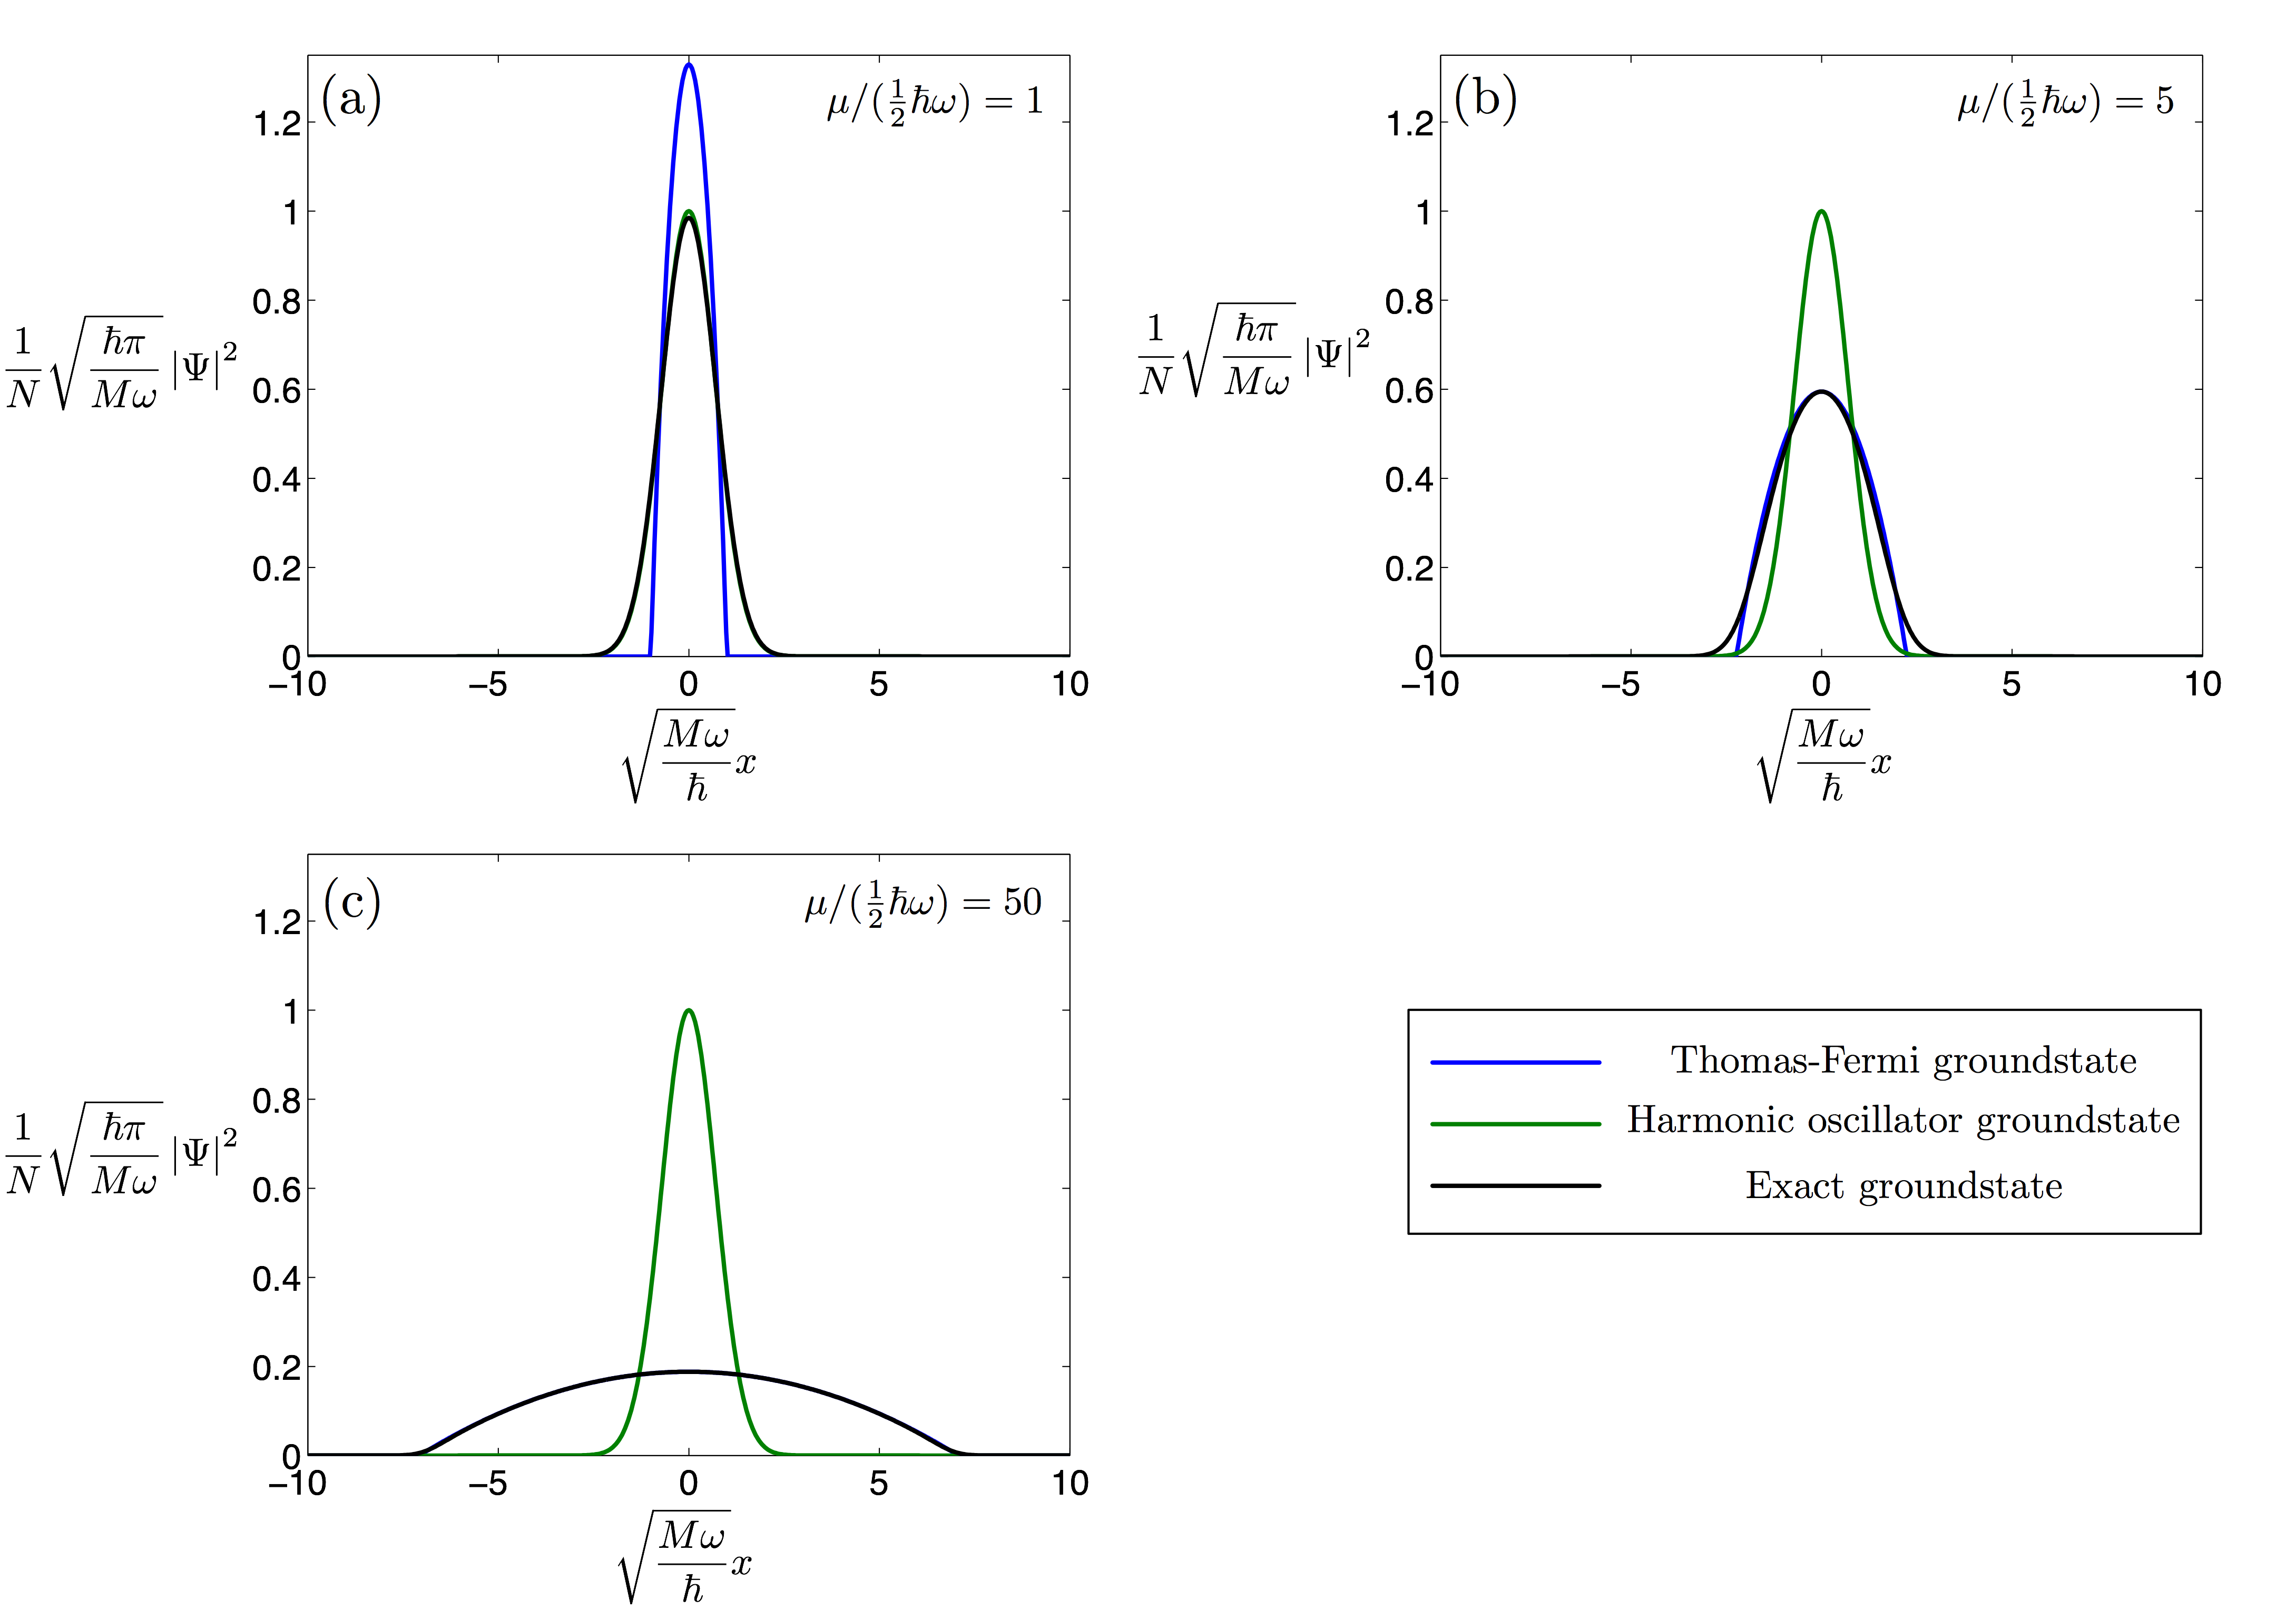
\includegraphics[width=14cm]{GroundStateComparison}
    \caption{Comparison of harmonic oscillator, Thomas-Fermi and exact one-dimensional groundstates in different regimes.  (a) $\mu / (\frac{1}{2} \hbar \omega) = 1$, (b) $\mu / (\frac{1}{2} \hbar \omega) = 5$, (c) $\mu / (\frac{1}{2} \hbar \omega) = 50$.}
    \label{BackgroundTheory:GroundStateComparison}
\end{figure}

A comparison of the harmonic oscillator and Thomas-Fermi groundstates is given in \figureref{BackgroundTheory:GroundStateComparison}.  The density profile of the Thomas-Fermi wavefunction is that of a truncated inverted parabola.  Near the edge of the wavefunction the Thomas-Fermi approximation breaks down.  There, the nonlinear term is smaller, and the kinetic energy term is larger.  In this region, the density profile of the exact groundstate decays smoothly due to the kinetic energy term.  The Thomas-Fermi profile instead has a discontinuous first derivative.  This discontinuity gives rise to a well-defined condensate radius in each dimension given by
\begin{align}
    r_\text{TF} &= \frac{1}{\omega_r} \sqrt{\frac{2 \mu}{M}},
\end{align}
where $\omega_r$ is the trapping frequency of that dimension.

The Thomas-Fermi approximation is useful as a simple description of the condensate when other parts of the system are of primary interest (it is used in this manner in the next section), or as an initial guess when finding the true groundstate of the system numerically.

\subsection{Application: Transverse profile of the atom laser}
\label{BackgroundTheory:TransverseProfile}

As discussed in \sectionref{Introduction:PhotonAndAtomLasers}, an atom laser is formed by outcoupling from a condensate to produce a directional beam of highly coherent atoms.  These atom lasers show great promise for studies of fundamental physics and in high precision measurements \citep{Kasevich:2002}.  For these applications, it is crucial that the output mode of the atom laser is `clean' in both amplitude and phase to enable stable mode matching.  It is therefore important to understand what influences the transverse profile of an atom laser.  In this section, we demonstrate the application of the Gross-Pitaevskii equation to this problem.  The results presented here have been published in \citet{Dall:2007}.

\parasep

For a magnetically-trapped condensate in an $F=1$ manifold, the atoms in one of the $m_F$ Zeeman levels are trapped (the low-field seeking level, either $m_F=1$ as in metastable Helium or $m_F=-1$ as in \nucl{87}{Rb}), the atoms in the $m_F=0$ level experience no magnetic trapping potential to first order (and are referred to as `untrapped'), and the atoms in the level with $m_F$ having the opposite sign to the trapped state experience a repulsive potential and are referred to as `anti-trapped'.  For metastable Helium (He*), the potentials experienced by the three levels in a cylindrically-symmetric trap are
\begin{align}
    V_{m_F}(\vect{x}) &= m_F V_\text{trap}(\vect{x}) = m_F \frac{1}{2} M \left(\omega_r^2 x^2 + \omega_r^2 y^2 + \omega_z^2 z^2 \right). \label{BackgroundTheory:HeliumCylindricallySymmetricTrap}
\end{align}
These three levels are coupled by applying radio-frequency (rf) radiation resonant with the Zeeman splitting between the $m_F$ levels.  This Zeeman splitting is due to the magnetic trap (and a contribution from a constant bias field), and therefore the outcoupling process will be resonant along a surface of constant $V_\text{trap}(\vect{x})$.  Due to gravity, the centre of the condensate is a distance $g/\omega_y^2$ below the centre of the magnetic trap.  For weak traps, the outcoupling surfaces will be almost horizontal planes [see \figureref{BackgroundTheory:OutcouplingSurfaces}(a)], while for stronger traps, the outcoupling surfaces will be spheroids approximately concentric with the condensate [see \figureref{BackgroundTheory:OutcouplingSurfaces}(b)].  As we shall show, the shape of the outcoupling surface significantly impacts the transverse profile of the atom laser.

\begin{figure}
    \centering
    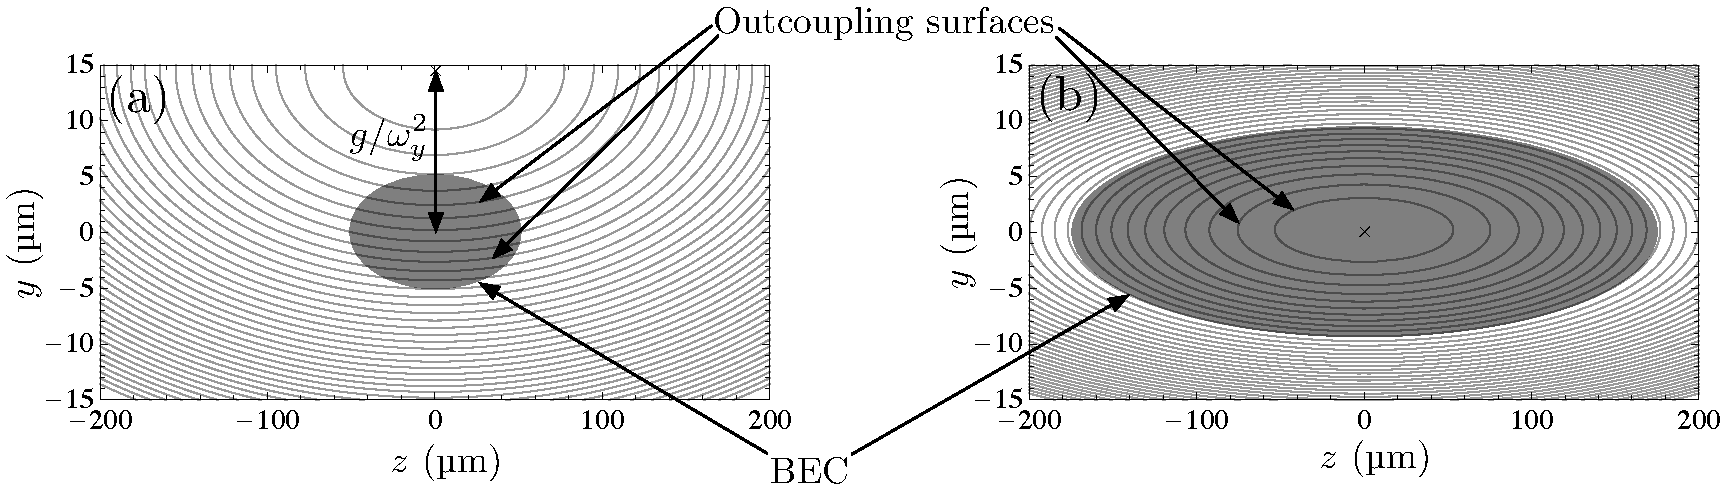
\includegraphics[width=15cm]{OutcouplingSurfaces}
    \caption{Outcoupling surfaces of condensates held in magnetic traps.  Pictured is the size of the Thomas-Fermi condensate and contours of the magnetic trap equally spaced in energy.  The origin of each coordinate system is the centre of the condensate, and the magnetic trap centres are marked by `$\times$'.  Figure (a) illustrates a condensate for typical parameters of the \nucl{87}{Rb} experiment at the Australian National University (ANU) \citep{Jeppesen:2008}; $N = 5 \times 10^5$ atoms, $\omega_r = 2 \pi \times \unit[130]{Hz}$, $\omega_z = 2 \pi \times \unit[13]{Hz}$.  The gravitational sag separating the centre of the condensate from the centre of the magnetic trap is $\Delta y = \unit[15]{\micro m}$.  Figure (b) illustrates a condensate for typical parameters of the He* experiment at the ANU \citep{Dall:2007a,Dall:2007}; $N = 2 \times 10^6$ atoms, $\omega_r = 2\pi \times \unit[1020]{Hz}$, $\omega_z = 2 \pi \times \unit[55]{Hz}$.  The gravitational sag separating the centre of the condensate from the centre of the magnetic trap is $\Delta y = \unit[0.2]{\micro m}$.  The acceleration due to gravity is in the $-y$ direction.  The aspect ratio of this figure is not 1:1 for reasons of clarity; the condensates are significantly more elongated than pictured.}
    \label{BackgroundTheory:OutcouplingSurfaces}
\end{figure}


The equations of motion for the system including the rf coupling are
\begin{subequations}
    \label{BackgroundTheory:AtomLaserF1}
    \begin{align}
        \begin{split}
            i \hbar \frac{\partial}{\partial t} \Psi_1(\vect{x}) &= \left[ - \frac{\hbar^2 \nabla^2}{2 M} + V_\text{trap}(\vect{x}) + M g y + U_\text{int}\left(\abs{\Psi_1}^2 + \abs{\Psi_0}^2 + \abs{\Psi_{-1}}^2\right)\right] \Psi_1(\vect{x})\\
            & + \hbar \Omega \Psi_0(\vect{x}),
        \end{split}\\
        \begin{split}
            i \hbar \frac{\partial}{\partial t} \Psi_0(\vect{x}) &= \left[ - \frac{\hbar^2 \nabla^2}{2 M} + M g y + U_\text{int} \left(\abs{\Psi_1}^2 + \abs{\Psi_0}^2 + \abs{\Psi_{-1}}^2\right)\right] \Psi_0(\vect{x})\\
            & + \hbar \Omega \Psi_1(\vect{x}) + \hbar \Omega \Psi_{-1}(\vect{x}),
        \end{split}\\
        \begin{split}
            i \hbar \frac{\partial}{\partial t} \Psi_{-1}(\vect{x}) &= \left[ - \frac{\hbar^2 \nabla^2}{2 M} - V_\text{trap}(\vect{x}) + M g y + U_\text{int}\left(\abs{\Psi_1}^2 + \abs{\Psi_0}^2 + \abs{\Psi_{-1}}^2\right)\right] \Psi_{-1}(\vect{x})\\
            & + \hbar \Omega \Psi_0(\vect{x}),
        \end{split}
    \end{align}
\end{subequations}
where $\Omega$ is the Rabi frequency, which is chosen to be real.

Initially, the condensate is in the ground state of the trapped $m_F=1$ state.  Once the outcoupling is turned on, the states are coupled and atoms are transferred to the $m_F=0$ and $m_F=-1$ levels.  In the limit of weak outcoupling, the atoms in the $m_F=0$ level leave the region in which outcoupling is resonant without being significantly coupled into the $m_F=-1$ level.  The $m_F=-1$ level is therefore relatively unpopulated and may be neglected.  It is the untrapped $m_F=0$ level that we are primarily interested in as the freely-falling atom laser forms in this level.

For short times, most of the atoms are in the $m_F=1$ level and we may use the Thomas-Fermi approximation to determine the effective potential seen by the untrapped $m_F=0$ atoms.  Inside the condensate, the effective potential for the untrapped atoms has contributions from gravity and interatomic interactions,
\begin{align}
    V_\text{eff}(\vect{x}) &= M g y + U_\text{int} \abs{\Psi_1(\vect{x})}^2 = M g y + \left(\mu - V_\text{trap}(\vect{x}) - M g y \right) \notag\\
    &= \mu - V_\text{trap}(\vect{x}).
\end{align}
This effective potential experienced by the untrapped atoms is a repulsive harmonic potential centred at the centre of the magnetic trap.  Once the atoms are outcoupled they therefore accelerate away from the centre of the magnetic trap until they reach the edge of the condensate, whereupon they fall under gravity.

There is a great difference in the behaviour of atoms outcoupled from a weak trap and from a tight trap.  If the outcoupling surfaces are almost horizontal planes [\figureref{BackgroundTheory:OutcouplingSurfaces}(a)], the atoms will be accelerated almost uniformly downwards.  If the outcoupling surfaces are prolate spheroids entirely contained within the condensate [\figureref{BackgroundTheory:OutcouplingSurfaces}(b)], atoms will be expelled in all directions away from the centre of the magnetic trap.  This difference is illustrated in \figureref{BackgroundTheory:HeliumTransverseProfile}, which displays the results of 3D GP simulations of the density of the atom laser in the region near the BEC in the cases of a weak trap [$\omega_r = 2\pi \times \unit[50]{Hz}$, $\omega_z = 2\pi \times\unit[50]{Hz}$; \figureref{BackgroundTheory:HeliumTransverseProfile}(a)] and a tight trap [$\omega_r = 2 \pi \times \unit[460]{Hz}$, $\omega_z = 2\pi \times \unit[50]{Hz}$; \figureref{BackgroundTheory:HeliumTransverseProfile}(b)].  

\begin{figure}
    \centering
    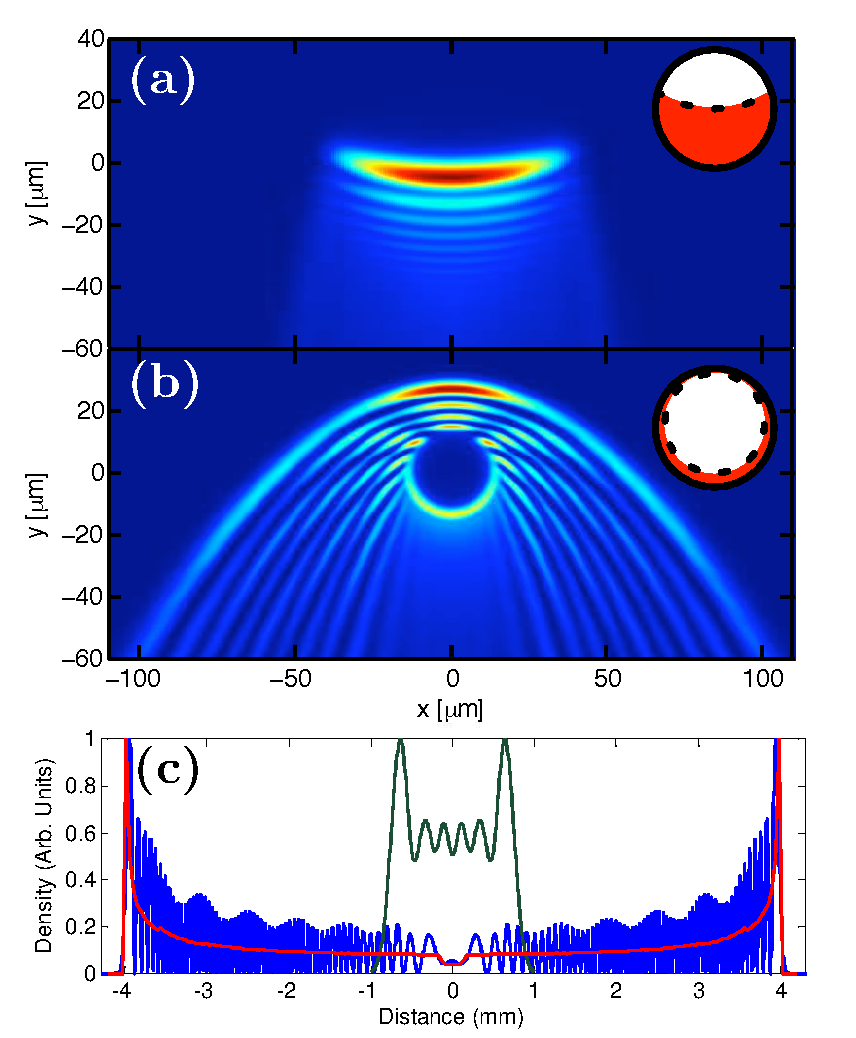
\includegraphics[width=10cm]{HeliumTransverseProfile}
    \caption{Near-field simulations of atom laser profiles, showing vastly different output dynamics depending on whether output-coupling takes place on (a) planes or on (b) prolate spheroids.  The output-coupling regions (dashed line), relative to the BEC (circle), used to create these plots are shown diagrammatically in the upper right corner of each plot.  In both cases the coordinate origin is the centre of the BEC is located at the origin.  The radial trapping frequencies of the two condensates are $\omega_r = 2 \pi \times \unit[50]{Hz}$ and $\omega_r = 2 \pi \times \unit[460]{Hz}$ for (a) and (b) respectively.  The resulting far field atom laser profiles as calculated at a detector $y=\unit[4]{cm}$ below the condensate for (a) and (b) are shown in (c).  The green profile results from the near field distribution shown in (a).  The blue and red profiles result from the near field distribution shown in (b) and are calculated using the Gross-Pitaevskii equation and classical mechanics respectively.  The classical simulation treats atoms as classical particles that begin on the outcoupling surface and are pushed from the BEC due to gravity and the mean field repulsion; the resulting `two-peak' structure is clearly visible.}
    \label{BackgroundTheory:HeliumTransverseProfile}
\end{figure}

It can be seen from the images of the near-field atom laser density in \figureref{BackgroundTheory:HeliumTransverseProfile}(a,~b) that the transverse profile of the atom laser has significantly greater structure when outcoupling from a tight trap than from a weak trap.  This difference is quite dramatic in the far field as shown in \figureref{BackgroundTheory:HeliumTransverseProfile}(c), although the atom laser produced from a weak trap also has interference fringes.  These interference fringes arise because it is possible for atoms outcoupled from different positions to have the same transverse momentum after leaving the condensate.  A large distance below the condensate these two atoms will occupy the same position and will interfere.  There are fewer interference fringes in the case of outcoupling from a weak trap as all atoms are accelerated downwards initially and therefore their maximum path length difference (and their maximum phase difference) will be smaller than if the atoms were outcoupled from a tight trap.  In the case of outcoupling from a tight trap, an atom that was initially accelerated upwards can have the same transverse momentum as an atom that was initially accelerated downwards.  The significantly larger maximum path length difference (and maximum phase difference) between these two atoms results in there being a greater number of interference fringes, as each $2\pi$ in the maximum phase difference corresponds to an interference fringe.  The maximum phase difference between two atoms arriving at the same location will vary from this maximum phase difference to zero.

While the fine structure of the transverse atom laser profile is caused by interference effects, the gross `double-peaked' structure is well-described classically [compare the red and blue lines of \figureref{BackgroundTheory:HeliumTransverseProfile}(c)].  The two peaks arise from the fact that, considered as a function of position on the outcoupling surface, there is a local maximum in the transverse momentum of the outcoupled atoms.  In the neighbourhood of this local maximum, the transverse momentum of outcoupled atoms will be approximately constant and therefore a greater number of atoms will contribute to the position on the detector corresponding to the maximum transverse momentum.  The `dip' in the centre of the transverse atom laser profile results from atoms which are outcoupled near the top of the outcoupling surface.  These atoms are initially accelerated upwards, but then fall back through the condensate.  This creates a shadowed region cast by the condensate, since atoms attempting to pass back through the condensate are pushed off axis due to the mean field repulsion.  This shadowed region is clearly visible below the condensate in \figureref{BackgroundTheory:HeliumTransverseProfile}(b).

\begin{figure}
    \centering
    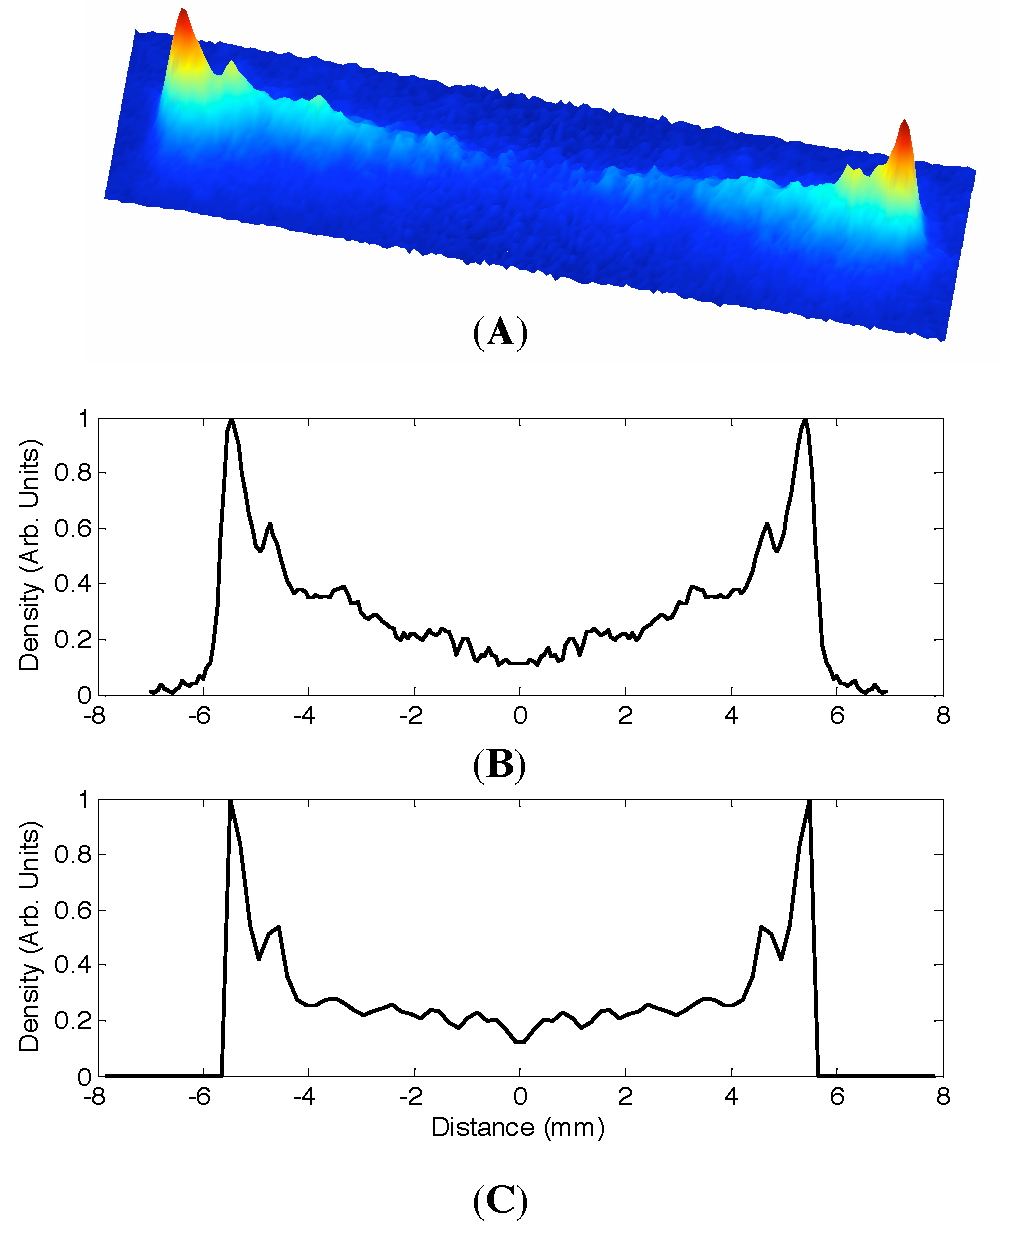
\includegraphics[width=10cm]{HeliumTransverseProfileExpTheoryComparison}
    \caption{Comparison of theory and experiment.  Upper trace shows an experimental 2D image of the transverse profile of an atom laser (image size is $\unit[13]{mm}$ by $\unit[3.4]{mm}$) taken $y=\unit[4]{cm}$ below the condensate.  Middle trace is an averaged profile taken through the centre of the 2D image.  Lower trace is the theoretical profile corresponding to the experimental conditions averaged over the detector resolution.}
    \label{BackgroundTheory:HeliumTransverseProfileExpTheoryComparison}
\end{figure}

\figureref{BackgroundTheory:HeliumTransverseProfileExpTheoryComparison} demonstrates that the results predicted by the Gross-Pitaevskii model of \eqref{BackgroundTheory:AtomLaserF1} are in good agreement with the experimental results from the Australian National University (ANU) He* experiment \citep{Dall:2007}.  The atom laser profile shown is for the case of outcoupling with Rabi frequency $\Omega = 2\pi\times \unit[50]{Hz}$ from the centre of a condensate of $N=2 \times 10^6$ atoms held in a magnetic trap with trapping frequencies $\omega_r = 2\pi \times \unit[50]{Hz}$ and $\omega_z = 2 \pi \times \unit[460]{Hz}$.  While the form of Eqs.~\eqref{BackgroundTheory:AtomLaserF1} is not particularly complicated, their solution can be numerically intensive.  Producing the theoretical profile of \figureref{BackgroundTheory:HeliumTransverseProfileExpTheoryComparison} required first solving \eqref{BackgroundTheory:AtomLaserF1} for the steady-state of the atom laser in the region near the condensate.  This  required 2000 hours of CPU time on a supercomputer, significantly longer than the simulations depicted in \figureref{BackgroundTheory:HeliumTransverseProfile}.  The reason for this difference is that in the case of \figureref{BackgroundTheory:HeliumTransverseProfileExpTheoryComparison}, atoms were outcoupled from the centre of the condensate, and therefore the atoms were moving faster and travelled higher after leaving the condensate.  This necessitated the use of a much finer grid to resolve the spatial oscillations of the atom laser on the length scale of the de Broglie wavelength, and a much larger grid to accommodate the atoms that travelled higher.  Some of the numerical tools and techniques used in simulations performed as part of this thesis are discussed in \sectionref{BackgroundTheory:NumericalTechniques}.

Although good agreement is seen between the predictions of the Gross-Pitaevskii model and the observed experimental profile, the presence of interference fringes on the atom laser will cause problems in mode matching the atom laser beam to another atom laser, as would be necessary in an atom interferometry experiment.  \figureref{BackgroundTheory:HeliumTransverseProfile} demonstrates that outcoupling from a weaker trap improves the transverse profile, making it closer to an ideal Gaussian beam.  It is also possible to improve the transverse mode by outcoupling closer to the bottom of the trap \citep{Riou:2006fk}, however this comes at the cost of reduced flux and a higher sensitivity to technical noise in the frequency of the outcoupling radiation \citep{Robins:2005uq}.  Other options for improving the transverse profile include using a multiphoton Raman outcoupling process \citep{Hagley:1999dz,Ruostekoski:2003,Jeppesen:2008} or guiding the atom laser optically \citep{Guerin:2006mz,Couvert:2008,Dall:2010}.  This last possibility, however, may introduce sufficient noise due to fluctuations in the waveguide to preclude its use in atom interferometry experiments \citep{Le-Coq:2006}.

\section{Loss processes and the master equation}

We are not always interested in the entirety of an interacting system; frequently it is only a small part of a system that is of interest.  For example, in \sectionref{BackgroundTheory:GrossPitaevskiiEquation} we considered a BEC and its environment, which was comprised of the almost empty atomic modes of the vacuum chamber in which the BEC was produced.  The environment is vastly larger than the BEC, both in terms of the number of available atomic modes, and in terms of the total occupation of those modes.  Condensates containing as many as $10^8$ \nucl{87}{Rb} atoms have been produced, however many more atoms ($\sim 10^{10}$) were initially in the trap before the evaporation process \citep{Streed:2006}.  The remaining atoms that are not part of the condensate comprise the environment.  While the entire system may be described by a many-body wavefunction, much of the information in this wavefunction will be describing the environment.  A description is necessary of the state of the condensate independent of the exact state of the environment.  The density matrix $\hat{\rho}$ provides that description \citep{Scully}.

As mentioned in \sectionref{BackgroundTheory:GrossPitaevskiiEquation}, a density matrix for a subsystem may be obtained by averaging (or tracing) over the degrees of freedom of the environment.  This simpler description fully describes the state of the subsystem when we are restricted to performing measurements only on that subsystem.  With this very natural restriction, it becomes impossible to distinguish otherwise distinct states of the entire system.  This indistinguishability is not fundamental; by performing measurements on the entire system the states may be distinguished.  The indistinguishability arises only due to our limited knowledge of the system.

Although not part of the subsystem of interest, the environment typically still influences the evolution of the subsystem.  For example, collisions with atoms in the environment will lead to losses from the condensate.  While knowledge of the state of the entire system is necessary to treat this exactly, if the interaction between the subsystem and its environment is sufficiently weak, and the subsystem is sufficiently small in comparison to its environment, the interaction may be treated perturbatively using the master equation technique originally derived in the context of quantum optics \citep{Senitzky:1960,Senitzky:1961}.  Specifically, for subsystem--environment interactions of the form
\begin{align}
    \hat{H}_\text{int} &= \hbar \sum_m \left(\hat{X}_m^\dagger \hat{\Gamma}_m^{\phantom{\dagger}} + \hat{X}_m^{\phantom{\dagger}} \hat{\Gamma}_m^\dagger \right), \label{BackgroundTheory:GeneralSubsystemEnvironmentCoupling}
\end{align}
where $\{\hat{X}_m\}$ are a set of bosonic annihilation operators acting only on the subsystem, and $\{\hat{\Gamma}_m\}$ are a set of operators acting only on the environment, the equation of motion for the density matrix gains the following term \citep[Chapter 5]{GardinerQN}:
\begin{align}
    \left.\frac{\partial}{\partial t} \hat{\rho}\right|_\text{int} &= \sum_m K_m \mathcal{D}[\hat{X}_m]\hat{\rho} + \sum_m G_m \mathcal{D}[\hat{X}_m^\dagger]\hat{\rho}, \label{BackgroundTheory:LindbladForm}
\end{align}
where $\mathcal{D}[\hat{a}]\hat{\rho} = \hat{a} \hat{\rho} \hat{a}^\dagger - \frac{1}{2}\left(\hat{a}^\dagger \hat{a} \hat{\rho} + \hat{\rho} \hat{a}^\dagger \hat{a} \right)$ is the decoherence superoperator, and the positive constants $K_m$ and $G_m$ depend on properties of the environment.  In the common case that the environment operators $\hat{\Gamma}_m$ are products of annihilation operators, the constants $G_m$ are zero if the modes of the environment are essentially unoccupied.

In the following section, the master equation will be used to model the process of Penning ionisation in metastable helium.

% A practical application of \eqref{BackgroundTheory:LindbladForm} is to the process of spontaneous emission.  Consider the case of a field of two-level atoms coupled by light.  Within certain approximations (see \sectionref{OpticalPumping:MultimodeModel} for details) the interaction Hamiltonian takes the form
% \begin{align}
%     \hat{H}_\text{int} &= \hbar \epsilon \int d \vect{x}\, \left(\hat{\Psi}_e^\dagger(\vect{x}) \hat{\Psi}_g^{\phantom{\dagger}}(\vect{x}) \hat{\Phi}_\text{ph}^{\phantom{\dagger}}(\vect{x}) + \hat{\Phi}_\text{ph}^\dagger(\vect{x}) \hat{\Psi}_g^\dagger(\vect{x}) \hat{\Psi}_e^{\phantom{\dagger}}(\vect{x})\right),
% \end{align}
% where $\epsilon$ is a coupling constant, $\hat{\Psi}_g$ and $\hat{\Psi}_e$ are the atomic field operators for the ground and excited states respectively, and $\hat{\Phi}_\text{ph}$ is the photon field operator.  If we are only interested in the behaviour of atoms in the excited state, we may consider $\hat{\Psi}_e$ to be our subsystem of interest with $\hat{\Psi}_g$ and $\hat{\Phi}_\text{ph}$ comprising the environment.  In this case, the subsystem operator $\hat{X}_m$ is $\hat{\Psi}_e$ and the environment operator $\hat{\Gamma}_m$ is $\hat{\Psi}_g \hat{\Phi}_\text{ph}$.  

\subsection{Application: Penning ionisation}
\label{BackgroundTheory:PenningIonisation}

The primary attraction of creating Bose-Einstein condensates of metastable helium atoms is that their large internal energy ($\unit[20]{eV}$) enables single-atom detection with high spatial (\micro m) and temporal resolution (ns). However, this large internal energy can be released when two metastable helium atoms collide, resulting in Penning ionisation (PI),
\begin{align}
    \label{BackgroundTheory:PenningIonisation}
    \text{He}^* + \text{He}^* & \rightarrow \left\{
        \begin{matrix}
            \text{He}^+ + \text{He} + e^-\\
            \text{He}_2^+ + e^-
        \end{matrix}\right..
\end{align}
While this process dominates for unpolarised cold samples such as magneto-optical traps~\citep{Bardou:1992}, it does not prohibit the formation of Bose-Einstein condensates as the process is suppressed by five orders of magnitude~\citep{Shlyapnikov:1994} in polarised samples.  This suppression is due to conservation of angular momentum. While the reactants each have a total angular momentum $s=1$, giving their combined total angular momentum as either $S=0$ or $S=2$ (assuming $s$-wave collisions), the products each have total angular momentum $s=\frac{1}{2}$ (in the case of $\text{He}^+$, $e^-$ and $\text{He}_2^+$) or $s=0$ (for $\text{He}$), giving the total angular momentum of the products as either $S=0$ or $S=1$. Hence spin polarised states having $S=2$, $m_S=\pm2$ cannot directly undergo the process \eqref{BackgroundTheory:PenningIonisation}.

In general as $S$ is conserved, any of the $S=2$ quasimolecule states will be prevented from directly undergoing PI. As collisions with nonzero relative angular momentum can be neglected at BEC temperatures~\citep{Venturi:2000,Stas:2006kx} (due to the atoms having insufficient energy to penetrate the centrifugal barrier), it is only the $S=0$ quasimolecule state that undergoes PI.

The Hamiltonian describing either of the processes \eqref{BackgroundTheory:PenningIonisation} will be of the form
\begin{align}
    \hat{H}_\text{int} &= \hbar \epsilon \int d \vect{x}\, \left(\hat{\Gamma}^\dagger(\vect{x})\hat{\Xi}_{S=0, m_S=0}^{\phantom{\dagger}}(\vect{x}) + \hat{\Xi}_{S=0, m_S=0}^\dagger (\vect{x}) \hat{\Gamma}(\vect{x}) \right), \label{BackgroundTheory:PIInteractionHamiltonian}
\end{align}
where $\epsilon$ is a spatially-independent coupling constant, $\hat{\Gamma}$ is a product of annihilation operators for the products of the PI process, and the $S=0$ quasimolecule state that undergoes PI is given by [see \eqref{BackgroundTheory:QuasimoleculeOperatorsDefinition}]
\begin{align}
    \hat{\Xi}_{S=0, m_S=0} &= \frac{1}{\sqrt{3}} \left( 2 \hat{\Psi}_1 \hat{\Psi}_{-1} - \hat{\Psi}_0 \hat{\Psi}_0\right).
\end{align}

As we are only interested in the metastable helium atoms, and not the products of the PI process, $\hat{\Xi}_{S=0, m_S=0}$ is the subsystem operator of the interaction Hamiltonian \eqref{BackgroundTheory:PIInteractionHamiltonian}, and $\hat{\Gamma}$ is the environment operator.  As the environment operator is of the form of a product of annihilation operators and the products of PI will have sufficient kinetic energy to leave the condensate rapidly (and therefore keep the $\hat{\Gamma}$ modes near the condensate unoccupied), the master equation term describing Penning ionisation must have the form
\begin{align}
    \left.\frac{d \hat{\rho}}{dt}\right|_\text{PI} &= \gamma_\text{PI} \int d \vect{x}\, \mathcal{D}\left[ \hat{\Xi}_{S=0, m_S=0}\right] \hat{\rho}, \label{BackgroundTheory:PenningIonisationMasterEquationTerm}
\end{align}
where $\gamma_\text{PI}$ is a positive rate constant.  An explicit form for this rate constant is obtained in \sectionref{PenningIonisationAppendix:MasterEquation}.  It is shown there that $\gamma_\text{PI} = \frac{9}{2} \Kunpol$, where $\Kunpol = \unit[7.7\times 10^{-17}]{m\textsuperscript{3}s\textsuperscript{-1}}$ is the rate constant for the production of ions due to Penning ionisation in an unpolarised thermal sample at $\unit[1]{\micro K}$~\citep{Stas:2006kx}.

\section{Beyond the Gross-Pitaevskii equation}
\label{BackgroundTheory:BeyondGrossPitaevskii}

In deriving the Gross-Pitaevskii equation, the atomic field $\hat{\Psi}(\vect{x})$ was separated into a classical component $\Psi(\vect{x})$ and a fluctuations operator $\delta\hat{\Psi}(\vect{x})$,
\begin{align}
    \hat{\Psi}(\vect{x}) &= \Psi(\vect{x}) + \delta\hat{\Psi}(\vect{x}),
\end{align}
where it was then assumed that the fluctuations operator was `small'.  This is the so-called semiclassical or mean-field approximation, which includes single-particle quantum mechanical effects such as interference and barrier-tunnelling.  This approximation neglects some of the more interesting quantum phenomena such as entanglement and squeezing \citep{Scully}.  This section discusses some techniques beyond the Gross-Pitaevskii equation that include these quantum statistical effects to varying levels of approximation.  

There are two classes of methods that go beyond semiclassical approximations.  In the first class of methods, the state of the system is quite general, and an expansion is performed in the evolution of the system, which is truncated at a certain level.  The stochastic phase-space methods are the most common of this class, and are discussed in  \sectionref{BackgroundTheory:StochasticPhaseSpaceMethods}.  In the second class of methods, an expansion is performed in the form of the system's state.  This expansion is truncated at some level, neglecting correlations above a certain order.  Requiring the state of the system to be of a certain form implicitly approximates the evolution of the system as well, however these approximations are of a different kind to those of the first class.  The Bogoliubov-type methods are representative of the second class of methods, and are discussed in \sectionref{BackgroundTheory:BogoliubovMethods}.

% Note that Karen's recent +P / HFB (bog?) hybrid is a cross-over between these two classes.


\subsection{Stochastic phase-space methods}
\label{BackgroundTheory:StochasticPhaseSpaceMethods}

% c-number methods?

Phase-space representations are real-valued functions that are an alternative description of the state of the system, fully equivalent to the density matrix $\hat{\rho}$.  In addition to being useful pictorial representations of the state of a system, these phase-space representations can be used to derive stochastic methods for describing the evolution of the system.

There are several phase-space representations, the most common being the P, Q and Wigner distributions.  Each of these represent the state of the system in terms of coherent states.  This is mostly clearly seen for the P-function,
\begin{align}
    \hat{\rho} &= \int d \alpha\, P(\alpha) \ketbra{\alpha}{\alpha}, \label{BackgroundTheory:PFunction}
\end{align}
where $P(\alpha)$ is the P-function for the single-mode system described by the density matrix $\hat{\rho}$.  Every density matrix has a unique P-function representation.  This P-function representation fully describes the state of the system, and is completely equivalent to the density matrix itself.  

While the P-function is real, it is frequently pathological.  For example, the coherent state $\ket{\alpha_0}$ has the P-function representation
\begin{align}
    P(\alpha) &= \delta^2(\alpha - \alpha_0).
\end{align}
The Wigner and Q functions are significantly less pathological as they can be obtained by convolving the P-function with $\frac{2}{\pi}e^{-2 \abs{\alpha}^2}$ and $\frac{1}{\pi} e^{-\abs{\alpha}^2}$ respectively.  Despite this convolution, the Wigner and Q functions are also complete representations of the state of the system \citep{GardinerQN}.

Instead of considering the evolution of the density matrix directly, the stochastic phase-space methods aim to model the evolution of phase-space representations.  If the equation of motion for the phase-space representation is of the form of a Fokker-Planck equation \citep{GardinerHSM}, the phase-space representation may be interpreted as a classical probability distribution.  In this case, the evolution may be equivalently described using stochastic differential equations.  Expectation values can then be calculated as averages of appropriate quantities over \emph{independent} realisations of a stochastic differential equation, which requires significantly fewer computational resources than solving the Fokker-Planck equation directly.  

In the general case, it is desired to transform the Fokker-Planck equation
\begin{align}
    \frac{\partial}{\partial t}F(\vect{\alpha}, t) &= - \sum_j \frac{\partial}{\partial \alpha_j} A_j(\vect{\alpha}, t) F(\vect{\alpha}, t) + \frac{1}{2} \sum_{j, k} \frac{\partial}{\partial \alpha_j^{\phantom{*}}} \frac{\partial}{\partial \alpha_k^*} D_{j,k}(\vect{\alpha}, t) F(\vect{\alpha}, t), \label{BackgroundTheory:GeneralFokkerPlanckEquation}
\end{align}
into the Stratonovich stochastic differential equation \citep{GardinerHSM}
\begin{align}
    d \alpha_i &= A_i(\vect{\alpha}, t)\, dt  - \frac{1}{2} \sum_{j, k} B_{k, j}(\vect{\alpha}, t) \frac{\partial }{\partial \alpha_k}B_{i,j}(\vect{\alpha}, t) \, dt + \sum_j B_{i,j}(\vect{\alpha}, t) \,d W_j(t), \label{BackgroundTheory:GeneralStratonovichSDE}
\end{align}
where the matrix $\vect{B}(\vect{\alpha}, t)$ is defined by
\begin{align}
    \vect{D}(\vect{\alpha}, t) &= \vect{B}(\vect{\alpha}, t) \vect{B}^\dagger(\vect{\alpha}, t),
\end{align}
and the Wiener increments $d W_j(t)$ are independent real Gaussian random variables with zero mean satisfying
\begin{align}
    \overline{d W_i(t) dW_j(t')} = \delta_{i j}\delta(t - t'),
\end{align}
where $\overline{(\cdot)}$ denotes an average over the random variables.  This decomposition is guaranteed when the matrix $\vect{D}(\vect{\alpha}, t)$ has only positive eigenvalues~\citep{GardinerHSM}, and may be possible when this requirement is loosened to only nonnegative eigenvalues. Note that the sums in \eqref{BackgroundTheory:GeneralFokkerPlanckEquation} and \eqref{BackgroundTheory:GeneralStratonovichSDE} are defined to run over both the complex variables $\alpha_j^{\phantom{*}}$ and their conjugates $\alpha_j^*$.

The transformation of a Fokker-Planck equation into a stochastic differential equation can be physically interpreted as the macroscopic and microscopic views of the same process. For example, a Fokker-Planck equation can be used to model the probability distribution of positions and velocities of particles in a gas (macroscopic view), and the corresponding stochastic differential equation would describe the path taken by individual particles (microscopic view).  The macroscopic view is useful when it is the distribution of positions and velocities which is of interest, or if it is only a few moments that are of interest, when the equations of motion for those moments form a closed system (such as those describing an ideal gas). Frequently however, the equations of motion are not closed with that for each moment depending on a higher-order moment [for example \eqref{BackgroundTheory:ExpectationValueEvolution}], and an assumption must be made to close the system of equations (in the case of \eqref{BackgroundTheory:ExpectationValueEvolution}, that the system remains in a coherent state). 

The microscopic view is an alternative approach that is useful when two conditions are met. The first is that only a finite set of moments of the distribution are of interest, and not the distribution itself. The second is that the motion of the particles are independent of one another (although they may depend on moments of the distribution). That the particles' motions are independent is equivalent to the eigenvalues of $\vect{D}(\vect{\alpha}, t)$ being nonnegative. Positive eigenvalues of $\vect{D}(\vect{\alpha}, t)$ can be physically interpreted as corresponding to a diffusion process, which microscopically takes the form of Brownian motion. Negative eigenvalues, however, correspond to \emph{negative} diffusion, a highly singular process in which particles tend to drift toward one another\footnote{It should be noted that the existence of negative eigenvalues for the matrix $\vect{D}(\vect{\alpha}, t)$ does not imply that the \emph{solution} to the Fokker-Planck equation is singular. A good example of this is the equation of motion for the Q-function~\citep{Scully} of the anharmonic oscillator which is periodic in time, yet the corresponding $\vect{D}(\vect{\alpha}, t)$ matrix has positive and negative eigenvalues of equal magnitude.}.  In this case, the evolution of one realisation of \eqref{BackgroundTheory:GeneralStratonovichSDE} will depend on the local \emph{distribution}, violating the conditions stated above.  One solution to this problem is to increase the dimensionality of the Fokker-Planck equation, and use the additional freedom given by the auxiliary dimensions to ensure that motion in the larger space is purely diffusive (this approach is taken with the Positive-P representation~\citep{GardinerQN}).  While this technique is exact in the limit of an infinite number of realisations of the corresponding stochastic differential equation, it is typically limited by the existence of trajectories with arbitrarily large norm \citep{Gilchrist:1997fk}.  These trajectories significantly increase the sampling error in calculated observables.  This problem is particularly acute for BEC systems, as the atomic scattering process described by \eqref{BackgroundTheory:SimpleScattering} causes the stochastic sampling error to diverge exponentially \citep{Gilchrist:1997fk}.  Such doubled phase-space techniques can therefore only describe the evolution of the system for short times.

% The Fokker-Planck equation is a faster technique when it is the distribution that is of interest, however the stochastic unravelling is a faster technique when it is only a few moments that are of interest.

\subsubsection{Application: Anharmonic oscillator}

We now demonstrate the application of a stochastic phase-space method to the anharmonic oscillator, which is governed by the Hamiltonian
\begin{align}
    \hat{H} = \hbar \omega \hat{a}^\dagger \hat{a} + \frac{1}{2} \hbar \kappa \hat{a}^\dagger \hat{a}^\dagger \hat{a} \hat{a}. \label{BackgroundTheory:AnharmonicOscillator:Hamiltonian}
\end{align}
We wish to consider the evolution of the system with initial state $\ket{\Psi(0)} = \ket{\alpha_0}$.  This system can be solved exactly, and has the interesting feature that its two-time correlation function initially decays, but undergoes perfect revivals when $\kappa t = 2 \pi n$ for integral $n$.  The normalised two-time correlation function for this system is
\begin{align}
    \frac{1}{N}\abs{\mean{\hat{a}^\dagger(t) \hat{a}(0)}}^2 &= \exp \left\{2 N \left[\cos(\kappa t) - 1 \right] \right\}, \label{BackgroundTheory:AnharmonicOscillator:ExactTwoTimeCorrelationFunction}
\end{align}
where $N = \abs{\alpha_0}^2$.

In this thesis, we will only consider stochastic methods based on the Wigner distribution, which is defined by \citep{Scully}
\begin{align}
    W(\alpha) &= \frac{1}{\pi^2} \int d^2 \lambda\, \exp\left(-\lambda \alpha^* + \lambda^* \alpha\right) \Tr\left\{ \exp\left(\lambda \hat{a}^\dagger - \lambda^* \hat{a}\right) \hat{\rho} \right\}.
\end{align}
An equation of motion for the Wigner function can be obtained using the equation of motion for the density matrix
\begin{align}
    \frac{\partial}{\partial t} W(\alpha) &= \frac{1}{\pi^2} \int d^2 \lambda\, \exp\left(-\lambda \alpha^* + \lambda^* \alpha\right) \Tr\left\{ \exp\left(\lambda \hat{a}^\dagger - \lambda^* \hat{a}\right) \frac{\partial}{\partial t}\hat{\rho}\right\} \notag \\
    &= \frac{1}{\pi^2} \int d^2 \lambda\, \exp\left(-\lambda \alpha^* + \lambda^* \alpha\right) \Tr\left\{ \exp\left(\lambda \hat{a}^\dagger - \lambda^* \hat{a}\right) \frac{-i}{\hbar} \left[\hat{H},\, \hat{\rho} \right]\right\},
\end{align}
for evolution driven by a Hamiltonian $\hat{H}$.  The simplification of this expression is made easier through the application of the following operator correspondences \citep[\S 4.5]{GardinerQN}
\begin{subequations}
    \begin{align}
        \hat{a} \hat{\rho} &\leftrightarrow \left(\alpha + \frac{1}{2} \frac{\partial}{\partial \alpha^*} \right) W(\alpha), \\
        \hat{\rho} \hat{a} & \leftrightarrow \left(\alpha - \frac{1}{2} \frac{\partial}{\partial \alpha^*} \right) W(\alpha), \\
        \hat{a}^\dagger \hat{\rho} & \leftrightarrow \left( \alpha^* - \frac{1}{2} \frac{\partial}{\partial \alpha} \right) W(\alpha), \\
        \hat{\rho} \hat{a}^\dagger & \leftrightarrow \left( \alpha^* + \frac{1}{2} \frac{\partial}{\partial \alpha} \right) W(\alpha).
    \end{align}
\end{subequations}
These correspondences apply for general density matrix evolution, not only for evolution driven purely by a Hamiltonian (see, for example, \sectionref{PenningIonisationAppendix:TW}).

For the anharmonic oscillator Hamiltonian \eqref{BackgroundTheory:AnharmonicOscillator:Hamiltonian}, the evolution equation for the Wigner distribution is
\begin{align}
    \label{BackgroundTheory:AnharmonicOscillator:WignerEvolution}
    \begin{split}
        \frac{\partial}{\partial t} W(\alpha) &=  i\left( \frac{\partial}{\partial \alpha} \alpha - \frac{\partial}{\partial \alpha^*} \alpha^*\right) \left[\omega + \kappa\left(\abs{\alpha}^2 - 1\right) \right] W(\alpha)\\
        &-\frac{1}{4}i \kappa \left(\frac{\partial^2}{\partial \alpha^2}\frac{\partial}{\partial \alpha^*}\alpha - \frac{\partial^2}{\partial {\alpha^*}^2} \frac{\partial}{\partial \alpha} \alpha^*\right) W(\alpha).
    \end{split}
\end{align}
The third-order derivatives in this equation mean that it is not in the form of a Fokker-Planck equation [cf.\ \eqref{BackgroundTheory:GeneralFokkerPlanckEquation}], and therefore may not be transformed into stochastic differential equations.  However, if these higher-order derivatives are neglected the equation of motion will only contain first-order derivatives and may therefore be transformed into a stochastic differential equation.  In fact, due to the absence of second-order derivatives, there will be no noise term in the resulting stochastic differential equation.  The initial condition is, however, stochastic. 

The neglect of third and higher-order derivatives in the equation of motion for the Wigner distribution is known as the Truncated Wigner (TW) approximation.  This is an uncontrolled approximation in the sense that there is no explicit small parameter in which this approximation is an expansion in.  We can motivate this approximation in the present system by considering the initial state of the Wigner distribution,
\begin{align}
    W(\alpha, t=0) &= \frac{2}{\pi} \exp\left(- 2 \abs{\alpha - \alpha_0}^2\right). \label{BackgroundTheory:WignerFunctionCoherentState}
\end{align}
As $\alpha_0$ changes, the initial Wigner distribution simply translates.  For small times therefore, each derivative can be considered to be of size $O(1)$ in $\alpha_0$.  The relative importance of each term in \eqref{BackgroundTheory:AnharmonicOscillator:WignerEvolution} therefore solely depends on the powers of $\alpha$ and $\alpha^*$.  The size of $\alpha$ and $\alpha^*$ can be considered to be of the order of $O(\alpha_0)$, as it is only in the vicinity of $\alpha_0$ that the Wigner distribution is significantly different from zero (for small times).  The $\kappa$-dependent terms of \eqref{BackgroundTheory:AnharmonicOscillator:WignerEvolution} involving first-order derivatives therefore scale as $O(\abs{\alpha_0}^2 \alpha_0)$, while the $\kappa$-dependent terms involving third-order derivatives scale as $O(\alpha_0)$.  For sufficiently large $\alpha_0$, the third-order derivative terms in \eqref{BackgroundTheory:AnharmonicOscillator:WignerEvolution} can be neglected, at least for small times.  The accuracy of the Truncated Wigner approximation has been considered in great detail elsewhere \citep{Sinatra:2002lq,Norrie:2005fk,Norrie:2006vn,Norrie:2006kx,Polkovnikov:2003}.  In general it has been shown that it is a good approximation if the total occupation of the system is much greater than the number of available modes \citep{Norrie:2006vn}.  For the anharmonic oscillator, this requires $N = \abs{\alpha_0}^2 \gg 1$.

We continue now with the application of the Truncated Wigner method to the anharmonic oscillator.  With the third-order derivatives neglected, the Stratonovich stochastic differential equation describing the system is
\begin{align}
    d \alpha &= -i \left[\omega + \kappa \left(\abs{\alpha}^2 - 1\right) \right] \alpha \, dt. \label{BackgroundTheory:AnharmonicOscillator:SDE}
\end{align}
Although the evolution of this `stochastic' differential equation is deterministic, its initial condition is random, as it must sample the initial condition of the Wigner distribution \eqref{BackgroundTheory:WignerFunctionCoherentState}.  The initial condition of \eqref{BackgroundTheory:AnharmonicOscillator:SDE} is therefore
\begin{align}
    \alpha(0) &= \alpha_0 + \frac{1}{\sqrt{2}} \eta,
\end{align}
where $\eta$ is a complex Gaussian random variable satisfying
\begin{align}
    \overline{\eta} &= 0, & \overline{\eta \eta} &= 0, & \overline{\eta^* \eta} &= 1.
\end{align}
The noise term in the initial state can be considered to be adding, on average, half a `virtual' particle per mode to the system \citep{Scott:2007}.  These virtual particles represent the contribution of the vacuum fluctuations that is ignored in the Gross-Pitaevskii equation.

In principle, \eqref{BackgroundTheory:AnharmonicOscillator:SDE} can be simulated numerically to determine the dynamics of the system.  However, as it is of a particularly simple form, it may be integrated analytically.  Within the Truncated Wigner approximation, the normalised two-time correlation function of the anharmonic oscillator is
\begin{align}
    \frac{1}{N} \abs{ \mean{\hat{a}^\dagger(t) \hat{a}(0)}_\text{TW}}^2 &= \frac{16}{(4 + \kappa^2 t^2)^2} \exp\left(\frac{- 4 N \kappa^2 t^2}{4 + \kappa^2 t^2} \right).
\end{align}
A comparison of the exact and truncated solutions is given in \figureref{BackgroundTheory:TwoTimeTWComparison}.

\begin{figure}
    \centering
    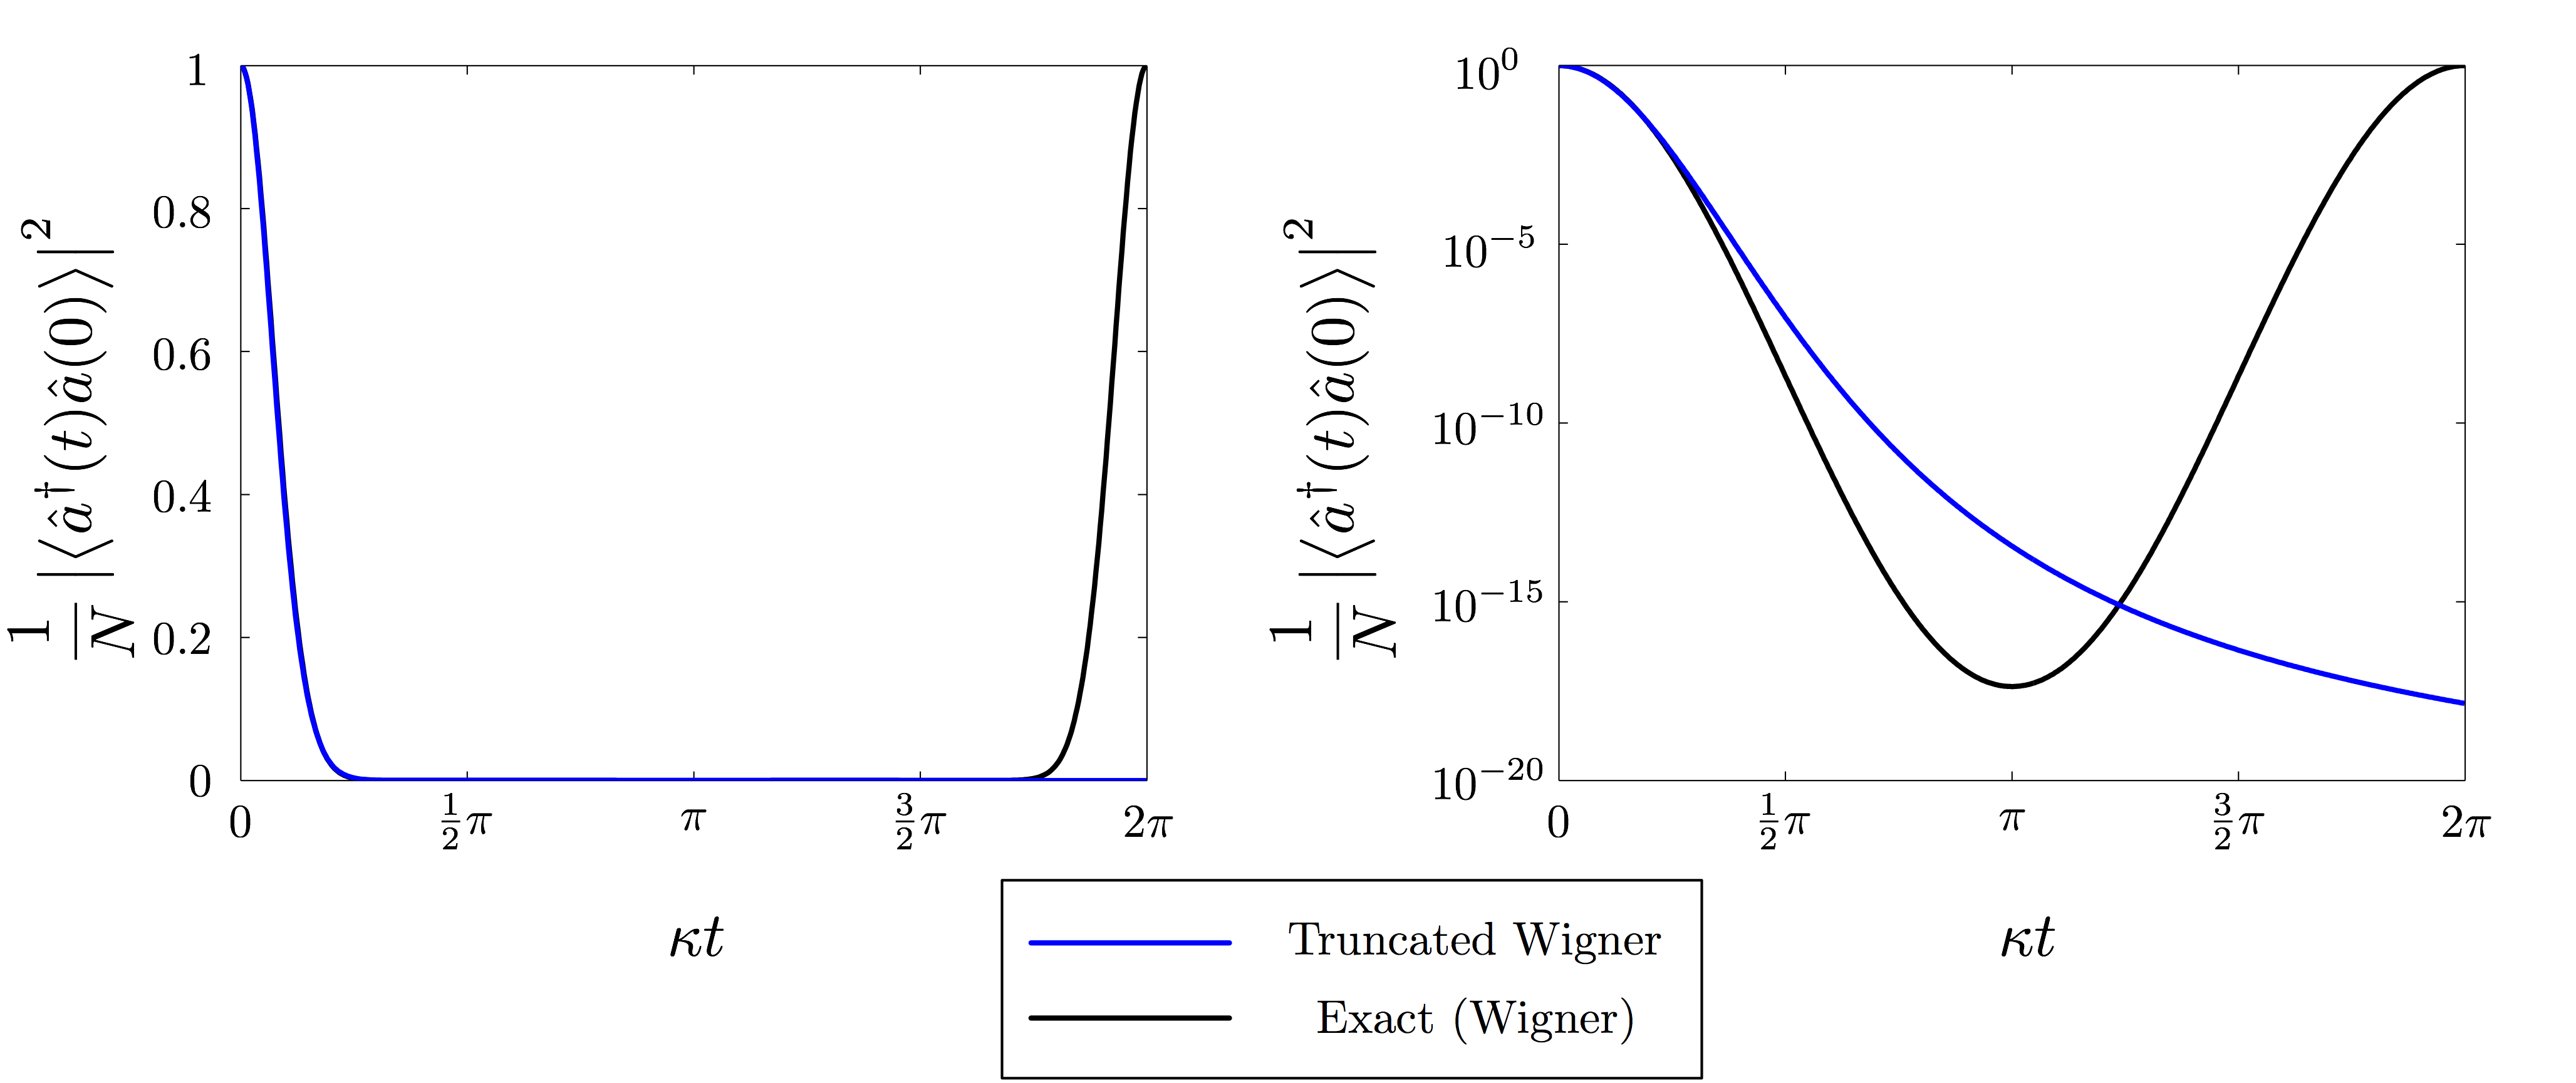
\includegraphics[width=15cm]{TwoTimeTWComparison}
    \caption{
        Comparison of Truncated Wigner with the exact solution for the two-time correlation function of the anharmonic oscillator.  The exact solution (black) for the two-time correlation function exhibits revivals every $\kappa t = 2\pi$, while the Truncated Wigner solution (blue) does not.  The Truncated Wigner solution, however, is in good agreement with the exact solution for the collapse of the correlation function.  The left and right figures illustrate the normalised two-time correlation function on linear and logarithmic scales respectively.  The initial condition was $\alpha_0 = \sqrt{10}$. \label{BackgroundTheory:TwoTimeTWComparison}
    }
\end{figure}

The good agreement between the Truncated Wigner and exact results in \figureref{BackgroundTheory:TwoTimeTWComparison} for $\kappa t \lesssim \frac{\pi}{4}$ does not imply that the distributions themselves are approximately equal over this time.  This is shown not to be the case in \figureref{BackgroundTheory:WignerTruncatedWignerComparison}, in which the Wigner and Truncated Wigner distributions for the anharmonic oscillator are compared.  Expectation values of higher-order moments will diverge from the exact solutions faster than those for lower-order moments.  The validity of Truncated Wigner therefore also depends on the moments that are to be calculated.  Typically, it is only second order moments such as $\mean{\hat{a}^\dagger \hat{a}}$ that are of interest. This is the case in this thesis.

\begin{figure}
    \centering
    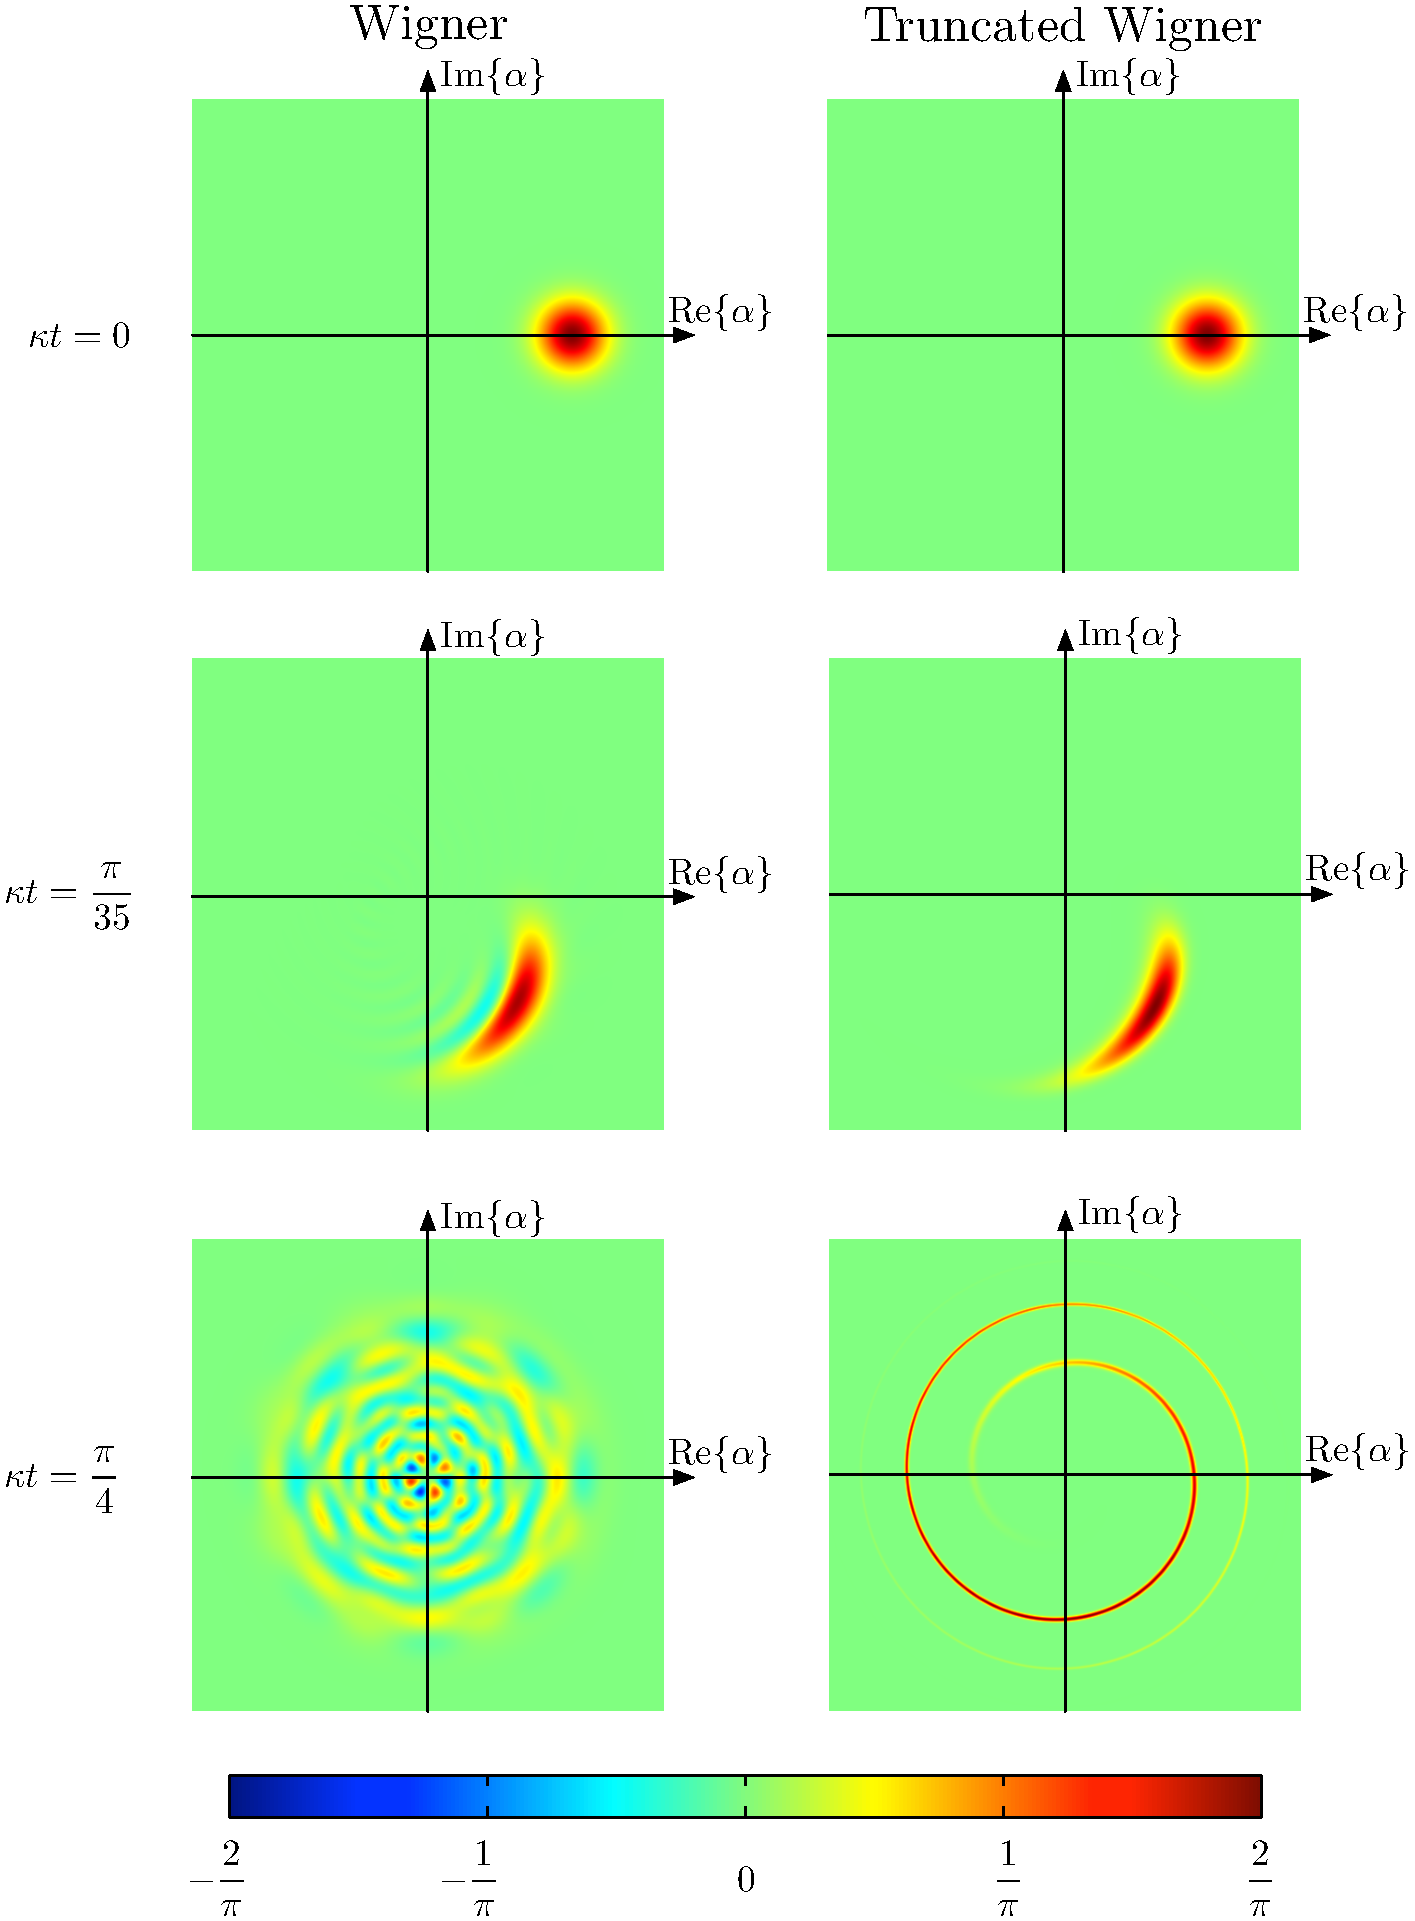
\includegraphics[width=14cm]{WignerTruncatedWignerComparison}
    \caption{
        Comparison of the Wigner and Truncated Wigner distributions for the anharmonic oscillator.  For short times, the two distributions are approximately equal (upper and middle rows), however for longer times (lower row) the Wigner distribution develops a significant negative components (blue).  As the Truncated Wigner distribution represents the probability distribution of the stochastic differential equation \eqref{BackgroundTheory:AnharmonicOscillator:SDE}, it remains positive.  The initial condition was $\alpha_0 = \sqrt{10}$. \label{BackgroundTheory:WignerTruncatedWignerComparison}
    }
\end{figure}

\parasep

Stochastic phase-space methods were described as being an expansion in the evolution of the system with no restriction on the state of the system.  The expansion in the evolution occurs at the level of the equation of motion for the phase-space distribution.  For an unravelling in terms of stochastic differential equations to be possible, all derivatives in this equation above second order must be truncated.  Although the requirement that the Truncated Wigner distribution be non-negative does impose a restriction on the state of the system, this restriction is not necessary \citep{Hush:2010}.  \citet{Polkovnikov:2003} has shown explicitly that the Gross-Pitaevskii equation and the Truncated Wigner method can be considered to be the zeroth and first order terms in an expansion of the system dynamics in terms of its response to quantum fluctuations.  In principle, higher-order corrections can be included, however the computational requirements increase rapidly for each additional correction considered.

Although the application of the Truncated Wigner method considered in this section did not involve explicitly stochastic evolution, an application that does is discussed in \appendixref{PenningIonisationAppendix}.

\subsection{Bogoliubov-type methods}
\label{BackgroundTheory:BogoliubovMethods}

The Bogoliubov-type methods consider the evolution of a truncated expansion of the state of the system.  These methods begin by decomposing the atomic field operator $\hat{\Psi}$ in terms of a classical component $\Psi = \mean{\hat{\Psi}}$ and a fluctuations operator $\delta \hat{\Psi}$,
\begin{align}
    \hat{\Psi} &= \Psi + \delta \hat{\Psi}.
\end{align}
The equations of motion for $\Psi$ and $\delta\hat{\Psi}$ may be obtained from \eqref{BackgroundTheory:ExpectationValueEvolution} and \eqref{BackgroundTheory:LocalOperatorEvolution} respectively \citep{Proukakis:2008},
\begin{subequations}
    \label{BackgroundTheory:Bogoliubov:GeneralEvolutionEquations}
    \begin{align}
        \begin{split}
            i \hbar \frac{\partial}{\partial t} \Psi &= \left(- \frac{\hbar^2 \nabla^2}{2 M} + V(\vect{x}) + U_\text{int} \abs{\Psi}^2 + 2 U_\text{int} \mean{\delta\hat{\Psi}^\dagger \delta\hat{\Psi}} \right) \Psi\\
            & + U_\text{int} \left(\mean{\delta\hat{\Psi} \delta\hat{\Psi}} \Psi^* + \mean{\delta\hat{\Psi}^\dagger \delta\hat{\Psi} \delta\hat{\Psi}} \right),
        \end{split} \label{BackgroundTheory:Bogoliubov:OrderParameterEvolution}\\
        \begin{split}
            i \hbar \frac{\partial}{\partial t} \delta\hat{\Psi} &= \left(-\frac{\hbar^2 \nabla^2}{2 M} + V(\vect{x}) + 2 U_\text{int} \abs{\Psi}^2 \right)\delta \hat{\Psi} + U_\text{int} \Psi^2 \delta \hat{\Psi}^\dagger\\
            &+ 2 U_\text{int} \Psi \left(\delta\hat{\Psi}^\dagger\delta\hat{\Psi} - \mean{\delta\hat{\Psi}^\dagger\delta\hat{\Psi}} \right)+ U_\text{int} \Psi^* \left(\delta \hat{\Psi}\delta \hat{\Psi} - \mean{\delta \hat{\Psi}\delta \hat{\Psi}} \right)\\
            &+ U_\text{int} \left(\delta\hat{\Psi}^\dagger \delta\hat{\Psi} \delta\hat{\Psi} - \mean{\delta\hat{\Psi}^\dagger \delta\hat{\Psi} \delta\hat{\Psi}} \right).
        \end{split} \label{BackgroundTheory:Bogoliubov:FluctuationOperatorEvolution}
    \end{align}
\end{subequations}
These equations are completely equivalent to the operator equation of motion \eqref{BackgroundTheory:LocalOperatorEvolution}, and are therefore equally infeasible to simulate numerically.  An approximation is needed to proceed.

There are a variety of methods that approximate \eqref{BackgroundTheory:Bogoliubov:GeneralEvolutionEquations} to varying degrees.  An extensive discussion of these methods is given in \citep{Proukakis:2008}.  The simplest of these is the Bogoliubov method in which the mean-field evolution \eqref{BackgroundTheory:Bogoliubov:OrderParameterEvolution} is approximated by the Gross-Pitaevskii equation and all terms of second- or higher-order in $\delta\hat{\Psi}$ are neglected.  This approximation restricts the applicability of this simplest method to the zero-temperature limit, where the effect of the thermal cloud on the condensate is small.  In this limit, however, the equations of motion are of sufficiently simple form as to enable analytic results to be obtained.  The Bogoliubov method is discussed in greater detail in \sectionref{Peaks:ElementaryExcitations}, and used in \sectionref{Peaks:PerturbativeApproach} to determine the stability of a He* condensate to excitations.

While the Bogoliubov method is useful in the zero-temperature limit, it does not consider effects such as scattering between the condensate and thermal fractions that are significant at higher temperatures.  In this limit, more accurate methods based on \eqref{BackgroundTheory:Bogoliubov:GeneralEvolutionEquations} such as the Hartree-Fock and Hartree-Fock-Bogoliubov methods are necessary.  These methods expand the state in terms of moments of the fluctuation operator.  This expansion is typically truncated at second-order, with the state described (in the case of Hartree-Fock-Bogoliubov theory) in terms of the moments
\begin{align*}
    \Psi(\vect{x}) &= \mean{\hat{\Psi}(\vect{x})}, & G_N(\vect{x}, \vect{x}') &= \mean{\delta\hat{\Psi}^\dagger(\vect{x}') \delta\hat{\Psi}(\vect{x})}, & G_A(\vect{x}, \vect{x}') &= \mean{\delta\hat{\Psi}(\vect{x}') \delta\hat{\Psi}(\vect{x})}.
\end{align*}
All higher-order moments are approximately expressed in terms of lower-order moments using Wick's theorem \citep{Wick:1950,Blaizot:1986}.  For example
\begin{align}
    \mean{\delta\hat{\Psi}^\dagger \delta\hat{\Psi}^\dagger \delta\hat{\Psi} \delta\hat{\Psi}} &\approx 2 \mean{\delta\hat{\Psi}^\dagger \delta\hat{\Psi}} \mean{\delta\hat{\Psi}^\dagger \delta\hat{\Psi}} + \mean{\delta\hat{\Psi}^\dagger \delta\hat{\Psi}^\dagger} \mean{\delta\hat{\Psi} \delta\hat{\Psi}}.
\end{align}

While these methods are appropriate at intermediate temperatures, other techniques are necessary near the phase transition at $T\sim T_c$.  Methods appropriate in this limit are discussed in the following section.

\subsection{Methods applicable near the critical temperature}

Near the critical temperature $T_c$, the system has a significant thermal fraction [see \eqref{BackgroundTheory:CondensateFractionHarmonicTrap}].  In this limit, scattering and particle-exchange between the condensed and thermal fractions are significant.  These processes are of particular importance when considering condensate formation and growth.  Simple models in which the condensate is described in terms of its occupation $N_0$, and the thermal cloud in terms of its energy distribution function $g(\varepsilon)$ have been quite successful in describing these processes \citep{Davis:2000vn,Bijlsma:2000}.  Such models use an extension of classical kinetic theory termed Quantum Kinetic theory \citep{Gardiner:1997tz,Jaksch:1997ug,Gardiner:1998wx,Jaksch:1998sj,Gardiner:2000ug,Lee:2000vs,Davis:2000vn}.  Quantum Kinetic theory is discussed in greater detail in \chapterref{KineticTheory}, in which it is used to describe the evaporation-driven pumping of a condensate.

More detailed models have since been developed that are applicable where the spatial dynamics of either the condensate or thermal cloud is important.  These include the $c$-field methods such as the (Stochastic) Projected Gross-Pitaevskii equation \citep{Blakie:2008a}, and the ZNG theory \citep{Zaremba:1999,Proukakis:2008}.  The former includes the statistics of the thermal cloud which is critical in low-dimensional systems \citep{Blakie:2008a}, while the latter employs a simpler representation of the thermal cloud which is simpler to solve numerically \citep{Proukakis:2008}.

\section{Numerical Techniques}
\label{BackgroundTheory:NumericalTechniques}

Numerical calculations are a common and important part of theoretical (and frequently experimental) physics.  While methods for validating the convergence of calculations by comparing results for different grid- and time-step sizes are well-known and understood, other techniques are less commonly discussed.  I have chosen to discuss one of these, the use of absorbing boundary layers, in \sectionref{BackgroundTheory:AbsorbingBoundaryLayers}.  An unusual application of this technique is discussed in \sectionref{Peaks:AbsorbingBoundaryTricks}.

There are a large number of technical details that must be correct for a simulation to operate correctly.  Diagnosing and resolving these issues can be a very difficult and time-consuming process.  As a large number of the problems solved within quantum and atom optics fall into the class of initial-value (stochastic) partial differential equations, the vast majority of these simulations are very similar at a mathematical level.  To reduce the time required to develop these simulations, the computational package \XMDS\ \citep{Collecutt:2001} was created several years ago to take a high-level description of a problem and produce a low-level simulation that solves the problem.  I have benefitted greatly from this tool throughout my PhD, however some of its limitations required the creation of a successor to this tool.  I have developed the package \xpdeint\ to fill this role, and a discussion of its capabilities is given in \appendixref{ToolsAppendix}.

\subsection{Absorbing boundary layers}
\label{BackgroundTheory:AbsorbingBoundaryLayers}

To solve any partial differential equation numerically, it must be restricted to a finite domain with boundary conditions imposed at the edges\footnote{This requirement can be avoided when the solution's asymptotic behaviour is known \emph{a priori}, however this case will not be encountered in this thesis.}. For some systems, this poses no additional restriction over the original problem as they are explicitly defined over a finite domain and with the correct boundary conditions this constitutes the problem itself (for example electromagnetic wave propagation in a waveguide). Other systems are naturally restricted to a finite domain (for example a BEC in a trap) and will be unaffected by the imposition of the artificial boundary conditions. 

With the exception of systems defined over a finite domain, the choice of boundary conditions at the edges of the computational domain is an artificial one; while in many cases they permit physical interpretation, this interpretation does not usually correspond to the reality of the system under consideration. As an example, consider the case of an atom laser outcoupled from a BEC, which then falls freely under gravity (see \figureref{BackgroundTheory:HeliumTransverseProfile}). The natural domain for this problem is infinite, but to solve this system numerically it must be restricted to a finite domain. If periodic boundary conditions are used, when the atom laser falls off the bottom of the computational domain, it will reappear at the top and continue falling. If the wavefunction or its derivative is set to zero on the boundary, then the atom laser will reflect from the bottom of the domain. Each choice of boundary condition gives different results and none correspond to the correct behaviour in which the atom laser would simply leave the computational domain. A strategy is therefore needed to limit the effect of the choice of the boundary conditions on the solution.

A first simple strategy would be to choose the computational domain to be large enough such that no part of the atom laser beam will reach the edge of the domain over the time of interest. While effective, this strategy can be computationally expensive, and is particularly demanding in the presence of gravity. Under the influence of gravity, a classical particle starting from rest will travel a distance $d = \frac{1}{2}g t^2$ in time $t$. Hence the size of the computational domain must increase as $t^2$. The spatial grid separation cannot remain constant however. As the velocity of the classical particle increases as $v = gt$, the mean wavelength of the particle $\displaystyle \lambda = \frac{\hbar}{Mv}$ must then decrease as $t^{-1}$.  To resolve the spatial dynamics of the atom laser, the step size between points must then decrease as $t^{-1}$. These two effects combine to give the scaling that the total number of spatial grid points required scales as $N_\text{pts} \propto t^3$. Choices of uniform or variable spacing for the grid will only differ by an overall constant factor in the number of points required by this strategy; such choices cannot change the overall scaling. A different strategy is needed.

In many circumstances it is the Bose-Einstein condensate and the outcoupling process that produces the atom laser that are of interest. In such situations the remainder of the atom laser that can no longer directly interact with the BEC must be prevented from doing so as a result of its unphysical interactions with the artificial boundary conditions. The solution used in the aforementioned strategy was to continue to model the atom laser, however this is not necessary. An alternative solution is to remove this part of the atom laser from the simulation in a way that has no effect on the BEC and the outcoupling process. One strategy that takes this approach is to add an \emph{absorbing boundary layer}~\citep{Kosloff:1986,Neuhasuer:1989} between the domain of interest and the artificial boundary conditions. This absorbing boundary layer takes the form of a negative imaginary potential, which must be chosen to be deep enough to strongly attenuate any wave traversing it and smooth enough to make the probability of reflection negligible. \figureref{BackgroundTheory:AbsorbingBoundarySchematic} illustrates this strategy. Through the use of an appropriate absorbing boundary layer, the computational domain used to solve the system need not change and the scaling problem discussed previously will not occur.

\begin{figure}
    \centering
    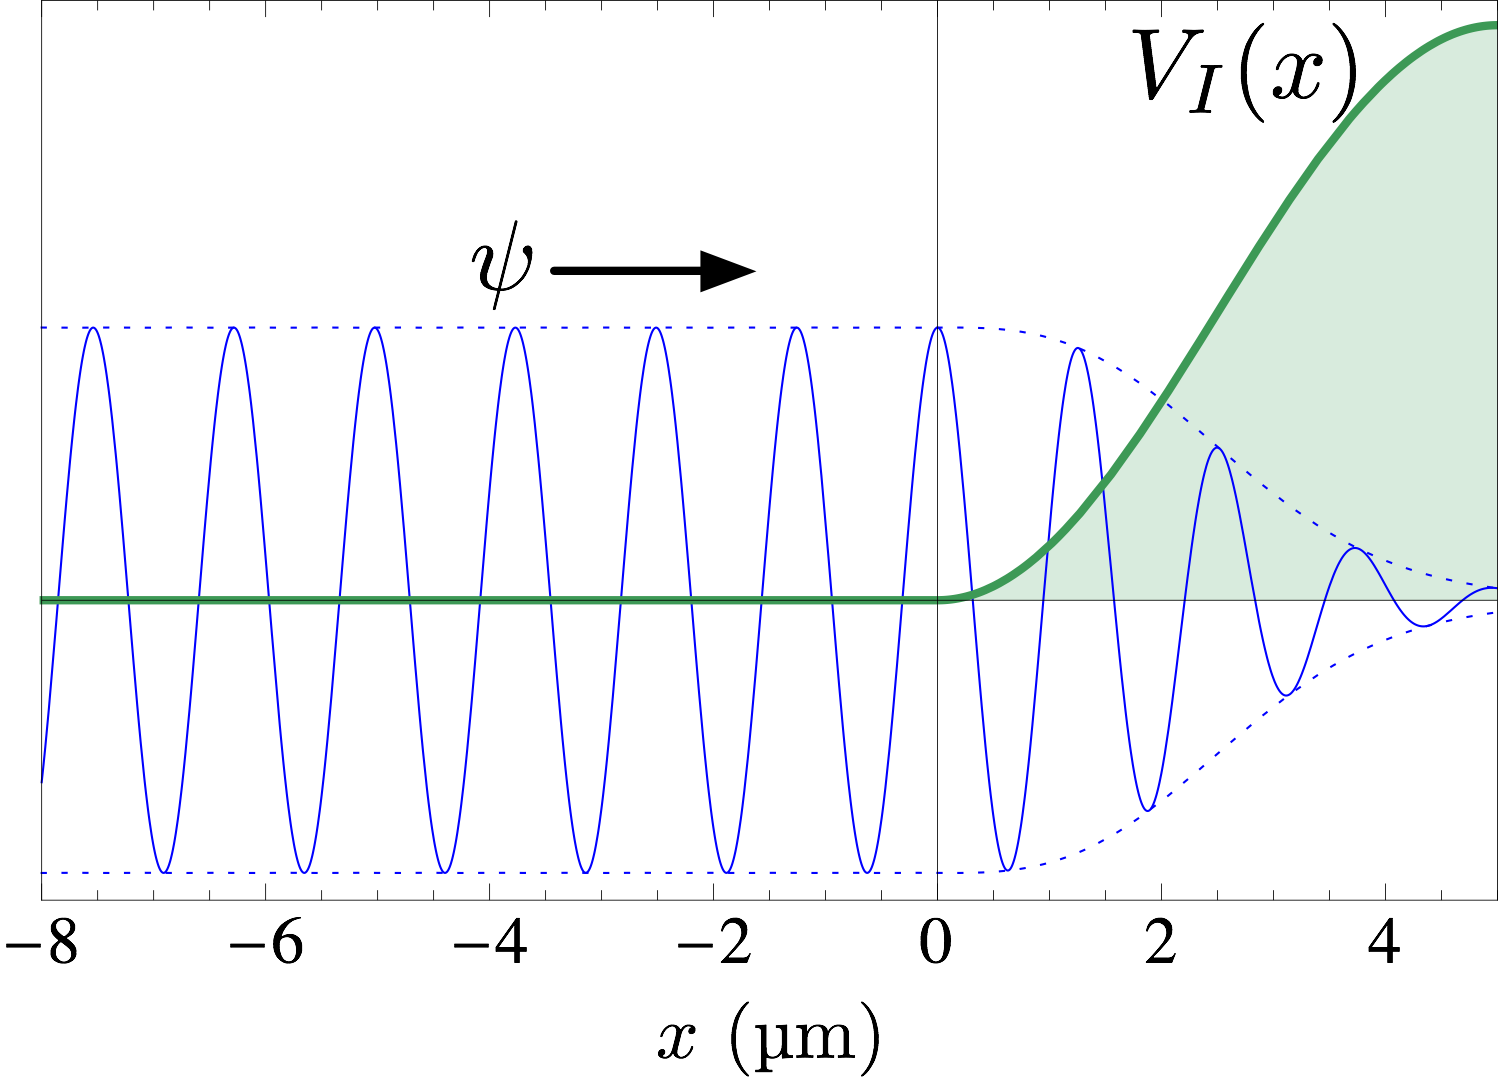
\includegraphics[width=8cm]{AbsorbingBoundarySchematic}
    \caption{
        \label{BackgroundTheory:AbsorbingBoundarySchematic}
        Schematic diagram illustrating the use of an absorbing boundary layer. A right-travelling wave is incident on the absorbing boundary layer, which is given by the potential $V(x) = -i V_I(x)$. The wave is attenuated as it crosses the absorbing boundary layer.
    }
\end{figure}

An absorbing boundary layer of finite thickness can only be effective over a finite range of incident wavenumbers. Incident wavefunctions with large wavelengths (low wavenumbers) will be reflected from the absorbing boundary layer due to the rapid variation in the potential over a wavelength. Incident wavenumbers with very short wavelengths (high wavenumbers) will be transmitted through the absorbing boundary layer due to the short amount of time spent in the absorbing boundary layer by any point on the phase-front.  Using this argument \citet{Neuhasuer:1989} showed that the approximate range of wavenumbers over which an absorbing boundary layer will be effective is
\begin{align}
    \label{BackgroundTheory:AbsorbingBoundaryKEffectiveRange}
    \left( \frac{M \overline{V_I}}{\hbar^2 \Delta x}\right)^{\frac{1}{3}} \ll k \ll \frac{4 M \overline{V_I} \Delta x}{\hbar^2},
\end{align}
where $\overline{V_I}$ is a representative value of $V_I(x)$. The maximum and minimum limits for the wavenumber are respectively due to the requirements of negligible transmission and reflection. Although cast in terms of the wavenumber, \eqref{BackgroundTheory:AbsorbingBoundaryKEffectiveRange} is equivalent to (26) in~\citep{Neuhasuer:1989}. While not its purpose, \sectionref{MethodsAppendix:MomentumDensityFluxExampleCalculation} demonstrates how to calculate the reflection and transmission coefficients as a function of wavenumber for arbitrary absorbing boundary layers.

The use of absorbing boundary layers must be slightly modified for use in phase-space methods such as those discussed in \sectionref{BackgroundTheory:StochasticPhaseSpaceMethods}. In these cases, simply adding an absorbing boundary layer to the potential would lead to unphysical results as the absorbing potential would not discriminate between real particles in a mode and the `virtual' particles which represent the fundamental vacuum fluctuations inherent in the field. An appropriate way of handling this problem is to add a position-dependent loss term to the master equation of the form
\begin{align}
    \label{BackgroundTheory:PhaseSpaceAbsorbingBoundaryLayer}
    \frac{d \hat{\rho}}{dt} &= \int d \vect{x}\, \frac{2}{\hbar}V_I(\vect{x})\mathcal{D}[\hat{\Psi}(\vect{x})]\hat{\rho},
\end{align}
where $\mathcal{D}$ is the usual decoherence superoperator. This master equation term leads to the same imaginary potential term in the equations of motion for the field operator with an additional noise term the for Truncated Wigner and Q function methods that restores the vacuum fluctuations that would otherwise be lost.

\parasep

In most of this thesis it is only the immediate vicinity of the BEC that is under consideration, and absorbing boundary layers are used to restrict the computational domain to this region.  As the use of absorbing boundary layers is a technical issue not related to the underlying physics, they are not included in equations of motion given in this thesis, but should be understood to be included when simulations are performed.  

% While direct application of absorbing boundary layers permit the study of dynamics near the BEC, in \chapterref{TransverseProfile} the transverse profile of the atom laser a large distance from the BEC is considered.  In this case a different strategy must be used to avoid the $N_\text{pts} \propto t^3$ scaling discussed above.  Such a strategy is discussed in \sectionref{TransverseProfile:DropGP}.

